\documentclass[12pt,letterpaper,reqno]{article}

% \usepackage{mathtools}
\usepackage{epsfig}
\usepackage{amsmath}
\usepackage{amssymb}
\usepackage{amsthm}
\usepackage{indentfirst}
\usepackage{xspace}
\usepackage{multirow}
\usepackage{hyperref}
\usepackage{xcolor}
\usepackage{verbatim}
\usepackage[letterpaper,margin=1in,headheight=15pt]{geometry}
\usepackage{mathpazo}
\usepackage{tikz-cd}
\usepackage{booktabs}
\usepackage{framed}
\usepackage{float}
\usepackage{thmtools}
\usepackage{dashrule}
\usepackage[missing=]{gitinfo2}
\usepackage{fancyhdr}
\usepackage{enumerate}
\usepackage{graphicx}
\usepackage{mathrsfs}
\usepackage{calligra}
\usepackage[titletoc,title]{appendix}
\usepackage{tikz}
\usetikzlibrary{decorations.markings}
\usetikzlibrary{arrows}

\definecolor{darkblue}{rgb}{0.1,0.1,0.7}
\definecolor{darkred}{rgb}{0.5,0.1,0.1}
\definecolor{darkgreen}{rgb}{0.0,0.42,0.06}
\hypersetup{colorlinks=true,urlcolor=darkred,linkcolor=darkblue,citecolor=darkred}
\definecolor{shadecolor}{rgb}{0.85,0.85,0.85}

% Bibliography formatting
\usepackage[bibstyle=authoryear-comp,labeldate=false,defernumbers=true,maxnames=20,uniquename=init,dashed=false,backend=biber,sorting=none]{biblatex}

\DeclareNameAlias{sortname}{first-last}

\DeclareFieldFormat{url}{\url{#1}}
\DeclareFieldFormat[article]{pages}{#1}
\DeclareFieldFormat[inproceedings]{pages}{\lowercase{pp.}#1}
\DeclareFieldFormat[incollection]{pages}{\lowercase{pp.}#1}
\DeclareFieldFormat[article]{volume}{\textbf{#1}}
\DeclareFieldFormat[article]{number}{(#1)}
\DeclareFieldFormat[article]{title}{\MakeCapital{#1}}
\DeclareFieldFormat[inproceedings]{title}{#1}
\DeclareFieldFormat{shorthandwidth}{#1}

% Don't use "In:" in bibliography. Omit urls from journal articles.
\DeclareBibliographyDriver{article}{%
  \usebibmacro{bibindex}%
  \usebibmacro{begentry}%
  \usebibmacro{author/editor}%
  \setunit{\labelnamepunct}\newblock
  \MakeSentenceCase{\usebibmacro{title}}%
  \newunit
  \printlist{language}%
  \newunit\newblock
  \usebibmacro{byauthor}%
  \newunit\newblock
  \usebibmacro{byeditor+others}%
  \newunit\newblock
  \printfield{version}%
  \newunit\newblock
%  \usebibmacro{in:}%
  \usebibmacro{journal+issuetitle}%
  \newunit\newblock
  \printfield{note}%
  \setunit{\bibpagespunct}%
  \printfield{pages}
  \newunit\newblock
  \usebibmacro{eprint}
  \newunit\newblock
  \printfield{addendum}%
  \newunit\newblock
  \usebibmacro{pageref}%
  \usebibmacro{finentry}}

% Remove dot between volume and number in journal articles.
\renewbibmacro*{journal+issuetitle}{%
  \usebibmacro{journal}%
  \setunit*{\addspace}%
  \iffieldundef{series}
    {}
    {\newunit
     \printfield{series}%
     \setunit{\addspace}}%
  \printfield{volume}%
%  \setunit*{\adddot}%
  \printfield{number}%
  \setunit{\addcomma\space}%
  \printfield{eid}%
  \setunit{\addspace}%
  \usebibmacro{issue+date}%
  \newunit\newblock
  \usebibmacro{issue}%
  \newunit}


% Bibliography categories
\def\makebibcategory#1#2{\DeclareBibliographyCategory{#1}\defbibheading{#1}{\section*{#2}}}
\makebibcategory{books}{Books}
\makebibcategory{papers}{Refereed research papers}
\makebibcategory{chapters}{Book chapters}
\makebibcategory{conferences}{Papers in conference proceedings}
\makebibcategory{techreports}{Unpublished working papers}
\makebibcategory{bookreviews}{Book reviews}
\makebibcategory{editorials}{Editorials}
\makebibcategory{phd}{PhD thesis}
\makebibcategory{subpapers}{Submitted papers}
\makebibcategory{curpapers}{Current projects}

\setlength{\bibitemsep}{2.65pt}
\setlength{\bibhang}{.8cm}
\renewcommand{\bibfont}{\small}

\renewcommand*{\bibitem}{\addtocounter{papers}{1}\item \mbox{}\hskip-0.85cm\hbox to 0.85cm{\hfill\arabic{papers}.~~}}
\defbibenvironment{bibliography}
{\list{}
  {\setlength{\leftmargin}{\bibhang}%
   \setlength{\itemsep}{\bibitemsep}%
   \setlength{\parsep}{\bibparsep}}}
{\endlist}
{\bibitem}

\newenvironment{publications}{\section{\LARGE Publications}\label{papersstart}\vspace*{0.2cm}\small
\titlespacing{\section}{0pt}{1.5ex}{1ex}\itemsep=0.00cm
}{\label{papersend}\addtocounter{sumpapers}{-1}\refstepcounter{sumpapers}\label{sumpapers}}

\def\printbib#1{\printbibliography[category=#1,heading=#1]\lastref{sumpapers}}

% Counters for keeping track of papers
\newcounter{papers}\setcounter{papers}{0}
\newcounter{sumpapers}\setcounter{sumpapers}{0}
\def\lastref#1{\addtocounter{#1}{\value{papers}}\setcounter{papers}{0}}

% theorem environments
\declaretheoremstyle[spaceabove=0.25cm,spacebelow=0.25cm,notefont=\normalfont\bfseries, notebraces={(}{)}]{theorem}
\declaretheoremstyle[spaceabove=0.25cm,spacebelow=0.25cm,bodyfont=\normalfont,notefont=\normalfont\bfseries, notebraces={(}{)}]{noital}
\declaretheoremstyle[spaceabove=0.25cm,spacebelow=0.25cm,bodyfont=\normalfont\color{darkgreen},notefont=\normalfont\bfseries, notebraces={(}{)}]{green}
\declaretheoremstyle[spaceabove=0.25cm,spacebelow=0.25cm,bodyfont=\normalfont,notefont=\normalfont\bfseries,qed=$\qedsymbol$,notebraces={(}{)}]{proofstyle}

\declaretheorem[name=Theorem,numberwithin=section,style=theorem]{thm}
\declaretheorem[name=Proposition,sibling=thm,style=theorem]{prop}
\declaretheorem[name=Corollary,sibling=thm,style=theorem]{cor}
\declaretheorem[name=Lemma,sibling=thm,style=theorem]{lem}
\declaretheorem[name=Definition,sibling=thm,style=noital]{defn}
\declaretheorem[name=Example,sibling=thm,style=noital]{example}
\declaretheorem[name=Exercise,numberwithin=section,style=green]{exercise}
\declaretheorem[name=Proof,style=proofstyle,numbered=no]{pf}

\numberwithin{equation}{section}


% macros for convenience
\newcommand{\tops}{\texorpdfstring}

\newcommand{\nid}{\noindent}

\newcommand{\fa}{{\mathfrak a}}
\newcommand{\fp}{{\mathfrak p}}
\newcommand{\fk}{{\mathfrak k}}
\newcommand{\fg}{{\mathfrak g}}
\newcommand{\fh}{{\mathfrak h}}
\newcommand{\fn}{{\mathfrak n}}
\newcommand{\fq}{{\mathfrak q}}
\newcommand{\fm}{{\mathfrak m}}
\newcommand{\fr}{{\mathfrak r}}
\newcommand{\fu}{{\mathfrak u}}
\newcommand{\fG}{{\mathfrak G}}

\newcommand{\cC}{\ensuremath{\mathcal C}}
\newcommand{\cG}{\ensuremath{\mathcal G}}
\newcommand{\cB}{\ensuremath{\mathcal B}}
\newcommand{\cL}{\ensuremath{\mathcal L}}
\newcommand{\cS}{\ensuremath{\mathcal S}}
\newcommand{\cF}{\ensuremath{\mathcal F}}
\newcommand{\cK}{\ensuremath{\mathcal K}}
\newcommand{\cZ}{\ensuremath{\mathcal Z}}
\newcommand{\cM}{\ensuremath{\mathcal M}}
\newcommand{\cN}{\ensuremath{\mathcal N}}
\newcommand{\cO}{\ensuremath{\mathcal O}}
\newcommand{\cH}{\ensuremath{\mathcal H}}
\newcommand{\cX}{\ensuremath{\mathcal X}}
\newcommand{\cY}{\ensuremath{\mathcal Y}}
\newcommand{\cA}{\ensuremath{\mathcal A}}
\newcommand{\cI}{\ensuremath{\mathcal I}}

\newcommand{\R}{\ensuremath{\mathbb R}}
\newcommand{\C}{\ensuremath{\mathbb C}}
\newcommand{\PP}{\ensuremath{\mathbb P}}
\newcommand{\Z}{\ensuremath{\mathbb Z}}
\newcommand{\Q}{\ensuremath{\mathbb Q}}
\newcommand{\A}{\ensuremath{\mathbb A}}
\newcommand{\bbH}{\ensuremath{\mathbb H}}
\newcommand{\bbI}{\ensuremath{\mathbb I}}
\newcommand{\bS}{\ensuremath{\mathbb S}}

\newcommand{\half}{\ensuremath{\frac{1}{2}}}
\newcommand{\qtr}{\ensuremath{\frac{1}{4}}}
\newcommand{\bq}{{\mathbf q}}
\newcommand{\N}{{\mathcal N}}
\newcommand{\F}{{\mathcal F}}
\newcommand{\HH}{{\mathcal H}}
\newcommand{\LL}{{\mathcal L}}
\newcommand{\RR}{{\mathcal R}}
\newcommand{\V}{{\mathcal V}}
\newcommand{\dirac}{\!\!\not\!\partial}
\newcommand{\Dirac}{\!\!\not\!\!D}
\newcommand{\cE}{{\mathcal E}}
\newcommand{\vs}{\not\!v}
\newcommand{\kahler}{K\"ahler\xspace}
\newcommand{\kq}{/\!\!/}
\newcommand{\kql}[1]{/\!\!/\!\!_#1\,}
\newcommand{\hk}{hyperk\"ahler\xspace}
\newcommand{\Hk}{Hyperk\"ahler\xspace}
\newcommand{\hkq}{/\!\!/\!\!/\!\!/}
\newcommand{\hkql}[1]{/\!\!/\!\!/\!\!/\!\!_#1\,}
\newcommand{\del}{\ensuremath{\partial}}
\newcommand{\delbar}{\ensuremath{\overline{\partial}}}
\newcommand{\I}{{\mathrm i}}
\newcommand{\J}{{\mathrm j}}
\newcommand{\K}{{\mathrm k}}
\newcommand{\e}{{\mathrm e}}
\newcommand\bid{{\mathbf 1}}
\newcommand{\de}{\mathrm{d}}
\newcommand{\ab}{\mathrm{ab}}
\newcommand{\vol}{\mathrm{vol}}
\renewcommand{\sf}{\mathrm{sf}}
\newcommand{\inst}{\mathrm{inst}}
\newcommand{\eff}{\mathrm{eff}}
\newcommand{\dR}{\mathrm{dR}}
\newcommand{\closed}{\mathrm{closed}}
\newcommand{\exact}{\mathrm{exact}}

\newcommand{\abs}[1]{\lvert#1\rvert}
\newcommand{\norm}[1]{\lVert#1\rVert}
\newcommand{\IP}[1]{\langle#1\rangle}
\newcommand{\DIP}[1]{\langle\!\langle#1\rangle\!\rangle}
\newcommand{\dwrt}[1]{\frac{\partial}{\partial#1}}
\newcommand{\eps}{\epsilon}
\newcommand{\simarrow}{\xrightarrow\sim}

\newcommand{\mmaref}[1]{}

\newcommand{\ti}[1]{\textit{#1}}
\newcommand{\tb}[1]{\textbf{#1}}
\newcommand{\lo}{\text{\calligra o}\,}
\newcommand{\dd}{\ensuremath{\mathscr{D}}}
\newcommand{\sgn}{\text{sgn}}


\DeclareMathOperator{\ad}{ad}
\DeclareMathOperator{\im}{Im}
\DeclareMathOperator{\re}{Re}
\DeclareMathOperator{\Tr}{Tr}
\DeclareMathOperator{\End}{End}
\DeclareMathOperator{\Hom}{Hom}
\DeclareMathOperator{\Aut}{Aut}
\DeclareMathOperator{\Sym}{Sym}
\DeclareMathOperator{\Lie}{Lie}
\DeclareMathOperator{\diag}{diag}
\DeclareMathOperator{\Bun}{Bun}
\DeclareMathOperator{\Vect}{Vect}
\DeclareMathOperator{\Span}{Span}
\DeclareMathOperator{\grad}{grad}
\DeclareMathOperator{\rank}{rank}
\DeclareMathOperator{\ind}{ind}
\DeclareMathOperator{\coker}{coker}
\DeclareMathOperator{\Jac}{Jac}
\DeclareMathOperator{\Hol}{Hol}
\DeclareMathOperator{\gr}{gr}

\newcommand{\insfig}[2]{

\medskip
\noindent
\begin{minipage}{\linewidth}

\makebox[\linewidth]{\includegraphics[keepaspectratio=true,scale=#2]{figures/#1-crop.pdf}}

\end{minipage}
\medskip

}


% \newcommand{\insfig}[2]{\begin{figure}[htbp] \centering \includegraphics[scale=#2]{figures/#1-crop.pdf} \label{fig:#1} \end{figure}}
% syntax: \insfig{name}{0.5}{caption}

\newcommand{\fixme}[1]{{\color{orange}{[#1]}}}
\newcommand{\currentposition}{{\color{blue} \noindent\makebox[\linewidth]{\hdashrule{\paperwidth}{1pt}{3mm}}}}

% \mathtoolsset{showonlyrefs}

\bibliography{mvc}

\begin{document}
\pagestyle{fancy}
\lhead{{\tiny \color{gray} \tt \gitAuthorIsoDate}}
\chead{\tiny \ti{Linear Algebra, GSMST 2018-2019}}
\rhead{{\tiny \color{gray} \tt \gitAbbrevHash}}
\renewcommand{\headrulewidth}{0.5pt}


\begin{center}
\tb{Multivariable Calculus \\
Semester 1: Linear Algebra} \\
Anderson Trimm \\
Gwinnett School of Mathematics, Science and Technology \\
\end{center}

{These are the notes for the Fall Semester 2019
of Multivariable Calculus at GSMST, which covers linear algebra. They will updated frequently throughout the semester. The latest PDF can always be accessed
at \small \url{https://github.com/atrimm/mvc/blob/master/Course%20Notes/linear_algebra_2019.pdf}.} Please email me with comments and corrections, or send them to me directly as pull requests to the source repository hosted at \small \url{https://github.com/atrimm/mvc}.

\tableofcontents
\renewcommand{\listtheoremname}{Quick reference}
\listoftheorems[onlynamed]

\newpage

%\setcounter{page}{1}
\section{Vectors and geometry}
\subsection{Physical motivation}
The earliest notion of a \emph{vector} comes from physics. In nature, we encounter certain physical quantities which cannot be uniquely specified by a number alone, but also depend on a direction in space. 

\begin{example}\label{ex:disp}
If the distance from town $A$ to town $B$ is 400 miles and we leave $A$ and travel at 50 miles per hour, then we will arrive at $B$ in 8 hours, but only if we travel in the direction from $A$ to $B$! Thus, displacement (400 mi, from $A$ to $B$) and velocity (50 mi/hr, from $A$ to $B$) are two examples of such physical quantities.
\end{example}
To distinguish physical quantities which depend on a numerical value alone from those which also depend on a direction, we make the following definitions. 
\begin{defn}[Vectors and scalars]
\begin{enumerate}[(a)] \hspace{10cm}
	\item A \emph{scalar} is a physical quantity which is uniquely specified by a numerical value alone.
	\item A \emph{vector} is a physical quantity which is uniquely specified by a numerical value, called its \emph{magnitude} or \emph{norm}, and a direction.
\end{enumerate}
\end{defn}

\begin{exercise}
Classify each of the following quantities are vector or scalar:
\begin{enumerate}[(a)]
	\item Force
	\item Temperature
	\item Mass
	\item Volume
	\item Acceleration
	\item Electric Charge
	\item Density
\end{enumerate}	
\end{exercise}

In the following sections, we will develop a mathematical model of vector and scalar quantities capable of modeling physical phenomena. As we will see, this model will have applications beyond physics as well.

\subsection{Mathematical model}
\subsubsection{Scalars}\label{sec:scalars}
While electric charges are observed in nature to take only integer values, other scalar quantities, such as mass and temperature, are found to take any \emph{real} value. Thus, in our model a scalar is simply a real number. We denote the set of all real numbers by $\mathbb{R}$. We will denote a scalar by a lower case latin letter, such as $x$.

\subsubsection{Vectors}
A vector quantity is uniquely specified by two pieces of information: a magnitude (which is a nonnegative real number) and a direction in three-dimensional space. We can therefore represent a vector geometrically as an \emph{arrow} (directed line segment) in space.  The arrow points in the direction specifying the vector while the length of the arrow represents the magnitude of the vector. For example, a force of 25 N directed at an angle of $45^\circ$ with respect to the positive $x$-axis is represented by the arrow 
\begin{figure}[h]
\begin{center}
	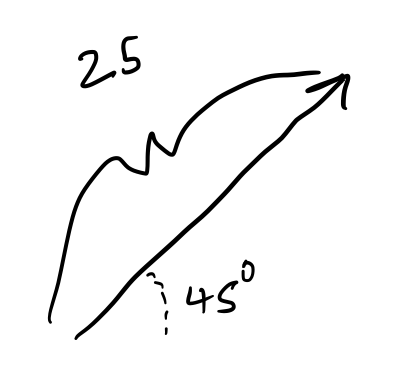
\includegraphics[scale=0.5]{figures_mvc/1stvector}
\end{center}
\end{figure}


 We will denote a vector by a boldface latin letter (either upper or lowercase), such as $\mathbf{x}$. When writing by hand, a more common notation is $\vec{x}$.

\subsubsection{Equality of vectors}
We will now discuss the notion of equivalence of two vectors. Recall first the equivalence of plane figures, say triangles. We consider two distinct triangles. Since the data defining a triangle are the side lengths and interior angle measures, any two triangles related by a transformation which leaves these unchanged represents an equivalent triangle; the only difference between them is the location in the plane. As you learned in basic algebra, any transformation of the plane which preserves lengths and angles can be written as a finite sequence of reflections, translations, and rotations and any two triangles related by such a transformation are said to be \emph{congruent}. 

Since the defining data of a vector is the magnitude and direction, we will agree that

\begin{defn}[Equality of vectors]
Two vectors are equal if they have the same magnitude and direction.	
\end{defn}
That is, two vectors are equal if they are represented by parallel line segments which have the same length and orientation. 

\begin{center}
	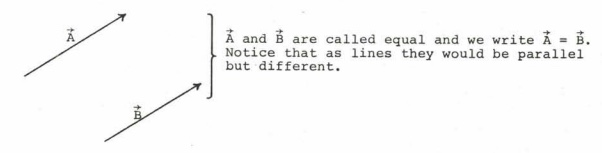
\includegraphics[scale=0.5]{figures_mvc/equal_vectors_new}
\end{center}
If two vectors $\mathbf{x}$ and $\mathbf{y}$ are equal, we will denote this by $\mathbf{x}=\mathbf{y}$.

It is important to note that we have defined equality of vectors so that \emph{location} in space does \emph{not} matter. As line segments, the two parallel arrows are congruent, \footnote{They are congruent simply because they have the same length; the fact that they are parallel or have the same orientation does not matter as far as congruence is concerned.} but still considered distinct due to their difference in location; on the other hand, as \emph{vectors} they are regarded as exactly the same vector. 

\subsection{Vector arithmetic}
We will now define operations involving vectors, whose motivation will come from physics. 

\subsubsection{Vector addition}
The most basic operation one can define on a set is a \emph{binary operation}, which is a rule for combining any two elements in the set to produce a third element in the set. \footnote{More formally, we write this as a map $V \times V \to V$, where $V \times V=\{(v,w) \mid v,w \in V\}$ denotes the set of all ordered pairs of elements of $V$, called the \emph{Cartesian product} of $V$ with itself.} There is a natural binary operation on the set of vectors, which is suggested by the \emph{force table} experiment in mechanics.

\begin{center}
	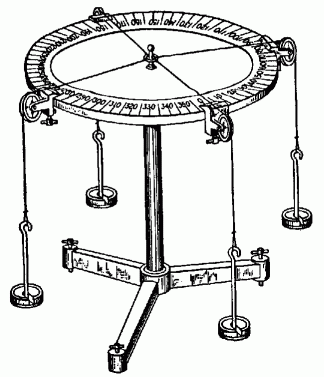
\includegraphics[scale=0.5]{figures_mvc/force_table_experiment_2}
\end{center}

In a force table experiment, strings are tied to a metal ring which is positioned at the center of the table. The strings are then suspended over pulleys which are fixed at known angles, and known masses hung from the ends of the strings. The pull of gravity on a given mass creates tension in the string which pulls on the ring. 

In an experiment in which \emph{two} strings are tied to the ring, the tension in each string gives rise to two forces pulling on the washer in different directions. However, the washer ultimately accelerates in a single direction, which is the direction of the \emph{net} (or \emph{total}) force acting on the ring. The rule for combining the two tension force vectors to produce the net force vector is exactly the binary operation we seek to define. 

To determine the net force, a third string is connected to the ring with mass and pulley position chosen so that the ring is in \emph{static equilibrium} (i.e., it does not move at all under the influence of these three forces). This vector is called the \emph{equilibrant} vector. By Newton's third law, the net force vector (also called the \emph{resultant} vector) is then the \emph{opposite} of the equilibrant vector, that is, it has the same magnitude and is directed along the same line, but with the opposite orientation.

\begin{center}
	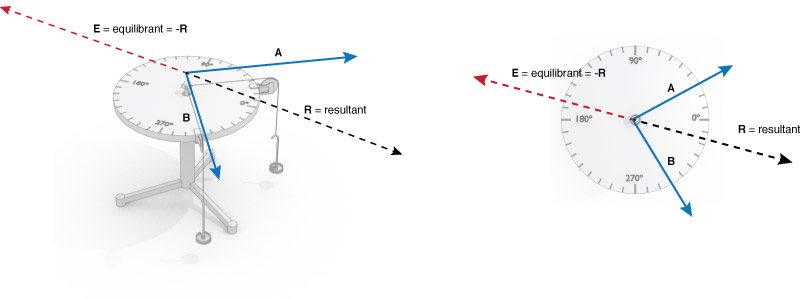
\includegraphics[scale=0.5]{figures_mvc/force-table-equi-res}
\end{center}

 We therefore define the \emph{sum} of two vectors as follows:
 
 \begin{defn}[Vector addition]
 	The \ti{sum} ${\bf v}+{\bf w}$ of two vectors ${\bf v}$ and ${\bf w}$ is the resultant vector of ${\bf v}$ and ${\bf w}$.
 \end{defn}
Note that when the two tension forces are along the \emph{same} direction (e.g., just add another mass on the same string), the resultant vector points in this same direction and has magnitude given by the sum of the magnitudes of the two tension vectors, and hence the addition of ${\bf v}$ and ${\bf w}$ reduces to addition of ordinary numbers in this special case. This is why we have decided to call this binary operation \emph{addition} and to continue to denote it by $+$; it can therefore be thought of as a \emph{generalization} of the ordinary addition of scalars. 
 
In terms of our geometric representation of vectors, the magnitude and direction of ${\bf v}+{\bf w}$ is determined as follows: Since the location of a vector is of no consequence (by our definition of equality of vectors), we may position the two vectors so that their initial points coincide. Then ${\bf v}$ and ${\bf w}$ form adjacent sides of a parallelogram, and the vector ${\bf v}+{\bf w}$ is the diagonal of the parallelogram, directed from the common initial point of ${\bf v}$ and ${\bf w}$ to the opposite vertex of the parallelogram, as shown below.	
\begin{center}
	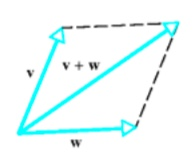
\includegraphics[scale=0.5]{figures_mvc/parallelogram_rule}
\end{center}
This is called the \ti{parallelogram rule} for vector addition. Since the opposite sides of a parallelogram are congruent and parallel, we can equivalently view ${\bf v}+{\bf w}$ as the result of positioning the initial point of ${\bf w}$ at the terminal point of ${\bf v}$ and drawing the arrow connecting the initial point of ${\bf v}$ to the terminal point of ${\bf w}$.

	\begin{center}
	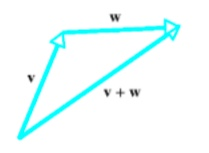
\includegraphics[scale=0.5]{figures_mvc/tip_to_tail}
\end{center}


This is called the \ti{triangle rule} or \ti{``tip to tail" rule} for vector addition. These two points of view are related by \ti{parallel translation}. To go from the first point of view to the second, we translate the initial point of ${\bf w}$ along ${\bf v}$, keeping ${\bf w}$ parallel to its original direction at all times. Accordingly, ${\bf v}+{\bf w}$ is also called the \ti{translation of ${\bf w}$ by ${\bf v}$}.
\begin{center}
	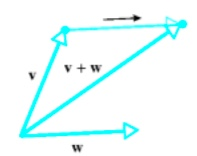
\includegraphics[scale=0.5]{figures_mvc/translation_of_v_by_w}
\end{center}

\begin{example}
There is another physical interpretation of this addition rule which agrees with our intuition. Suppose a person walks 10 steps in a north-easterly direction, and then turns and walks another 5 steps to the east. The vector $\mathbf{v}$ then represents his \emph{displacement} from his initial position, with the length of $\mathbf{v}$ being his distance from where he started, and the direction of $\mathbf{v}$ pointing in the direction in which he moved. Similarly, the vector $\mathbf{w}$ represents his displacement from his position after he traveled along the vector $\mathbf{v}$. Their sum, added according to the tip to tail rule, is his \emph{total} displacement from his initial position.	
\end{example}

Let us now use this geometric picture to determine the properties of vector addition. Recall that the addition operation defined on the set of real numbers satisfies the following properties: \footnote{Any set $G$ on which there is a binary operation $*$ which satisfies the first three of these properties is said to form a \emph{group} under $*$. One also says that $(G,*)$ is a group, or just that $G$ is a group if $*$ is understood. If the fourth property (commutativity) also holds, $G$ is said to form a \emph{commutative} (or \emph{abelian}) under $*$.}
\begin{enumerate}[(i)]
	\item Associativity: $(x+y)+z=x+(y+z)$ for all $x,y,z \in \mathbb{R}$.
	\item Existence of an additive identity: $\mathbb{R}$ contains an element 0 such that $0+x=x$ for every $x \in \mathbb{R}$.
	\item Existence of additive inverses: For every $x \in \mathbb{R}$, there exists and element $y \in \mathbb{R}$ such that $x+y=0$.
	\item Commutativity: $x+y=y+x$ for all $x,y \in \mathbb{R}$.
\end{enumerate}
We now consider each of these in turn. We consider commutativity first, since it is the simplest to analyze.

\begin{prop}[Vector addition is commutative]
	Vector addition is commutative. That is, 
	\begin{align*}
		{\bf v}+{\bf w}={\bf w}+{\bf v}
	\end{align*}
	for any two vectors ${\bf v}$ and ${\bf w}$, since each of these is the diagonal of the parallelogram whose edges are formed by $\mathbf{v}$ and $\mathbf{w}$.
\end{prop}

\begin{pf}
	We see from the two diagrams below that the translation of ${\bf w}$ by ${\bf v}$ is the same vector as the translation of ${\bf v}$ by ${\bf w}$.
\begin{center}
	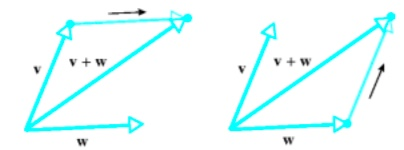
\includegraphics[scale=0.5]{figures_mvc/equivalence_of_vector_addition}
\end{center}

\end{pf}

\begin{prop}[Vector addition is associative]
	Vector addition is associative. That is, for any three vectors ${\bf u}, {\bf v},$ and ${\bf w}$, we have
	\begin{align*}
		{\bf u}+({\bf v}+{\bf w})=({\bf u}+{\bf v})+{\bf w}
	\end{align*}
We therefore denote both expressions by ${\bf u}+{\bf v}+{\bf w}$. 
\end{prop}

\begin{pf}
One can construct ${\bf u}+{\bf v}+{\bf w}$ by placing the vectors ``tip to tail" in succession and then drawing the vector from the initial point of ${\bf u}$ to the terminal point of ${\bf w}$. If the three vectors lie in the same plane, one can verify associativity from the diagram below.
\end{pf}

\begin{center}
	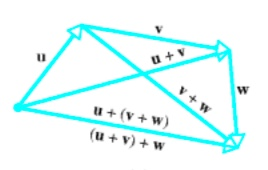
\includegraphics[scale=0.5]{figures_mvc/associativity_of_vector_addition}
\end{center}

If the three vectors do not all lie in the same plane, then when placed at the same initial point the vectors ${\bf u}, {\bf v},$ and ${\bf w}$ from adjacent edges of a \emph{parallelepiped}. \footnote{A parallelepiped is a polygon whose faces are parallelograms, with each pair of opposite sides parallel.} Translating these vectors and adding tip to tail, we see that ${\bf u}+{\bf v}+{\bf w}$ is the diagonal of this parallelepiped.

\begin{center}
	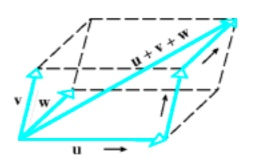
\includegraphics[scale=0.5]{figures_mvc/volume_of_parallelepiped_vectors}
\end{center}

\begin{cor}
The sum ${\bf v}_1+{\bf v}_2+\cdots + {\bf v}_k$ is independent of how the expression is bracketed.	
\end{cor}

\begin{pf}
We postpone the proof until we discuss vectors in coordinates in section \ref{sec:coords}, as the geometry is very complicated and difficult to analyze. In coordinates, this is seen to hold as a simple consequence of the fact that it holds for real numbers.
\end{pf}

Let us now check whether there is a vector which plays the role of an additive identity. That is, given any vector ${\bf b}$, is there a vector ${\bf 0}$ such that ${\bf b}+{\bf 0}={\bf b}$? Let us suppose there is such a vector ${\bf 0}$ and denote its magnitude by $r$. Let us now add ${\bf 0}$ to ${\bf b}$ by the tip-to-tail method. Since ${\bf 0}$ has magnitude $r$, ${\bf b}+{\bf 0}$ must lie on a circle of radius $r$ centered on the tip of ${\bf b}$. However, the condition ${\bf b}+{\bf 0}={\bf b}$ means that ${\bf b}+{\bf 0}$ must have the same magnitude and direction as ${\bf b}$, and there is no point on the circle for which this is true. This shows that there is no such vector ${\bf 0}$ with nonzero length. 
\begin{center}
	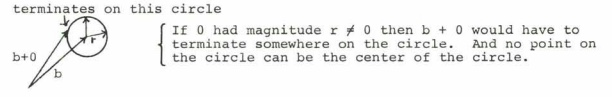
\includegraphics[scale=0.5]{figures_mvc/b_plus_zero_circle}
\end{center}

A vector of length zero, does not have a defined direction. Thus, there is a unique vector which acts as an additive identity with respect to vector addition.

\begin{defn}[The zero vector]
	The zero vector, which we denote by ${\bf 0}$, is the unique vector of magnitude zero.
\end{defn}

Finally, we want to investigate whether every vector has an additive inverse. That is, we want to determine if, when given any vector ${\bf a}$, we can find another vector ${\bf b}$ such that ${\bf a}+{\bf b}={\bf 0}$. Since the zero vector has zero length and since we add vectors from ``tip to tail", it follows that if ${\bf a}+{\bf b}={\bf 0}$, then the tail of ${\bf a}$ and the tip of ${\bf b}$ must coincide. Thus, any vector $\mathbf{a}$ has a \emph{unique} inverse, which we denote by $-\mathbf{a}$.   
\begin{center}
	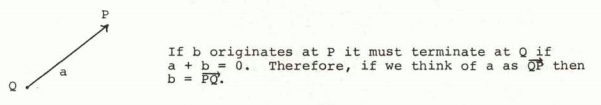
\includegraphics[scale=0.5]{figures_mvc/a_plus_b_equals_zero}
\end{center} 
\begin{defn}[Inverse of a vector]
The additive inverse of a vector ${\bf a}$ is the unique vector $-\mathfrak{a}$, which has the same magnitude as $\mathbf{a}$ and opposite orientation.
\end{defn}
In analogy with the equation $x+(-x)=0$ for real numbers, we denote the additive inverse of ${\bf a}$ by $-{\bf a}$, so that ${\bf a}+(-{\bf a})={\bf 0}$ for any vector ${\bf a}$. We may again agree, as in the case of numerical addition, to abbreviate ${\bf a}+(-{\bf b})$ as ${\bf a}-{\bf b}$, which allows us to define vector subtraction:

\begin{defn}[Vector subtraction]\label{def:vector_subtraction}
	The difference ${\bf a}-{\bf b}$ of two vectors ${\bf a}$ and ${\bf b}$ is the sum
	\begin{align*}
		{\bf a}-{\bf b}={\bf a}+(-{\bf b}).
	\end{align*}
\end{defn}
From this definition, we may view vector subtraction geometrically as follows: To form ${\bf a}-{\bf b}$,
\begin{enumerate}[(1)]
	\item Obtain $(-{\bf b})$ from ${\bf b}$ by reversing the direction of ${\bf b}$.
	\item Add ${\bf a}$ and $(-{\bf b})$ in the usual way, by placing the tail of $(-{\bf b})$ at the tip of ${\bf a}$. \footnote{Like numerical subtraction, vector subtraction is \ti{not} commutative, so the order matters here.}
\end{enumerate}

\begin{center}
	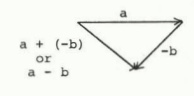
\includegraphics[scale=0.5]{figures_mvc/a_minus_b}
\end{center}

\begin{exercise}
Show that if $\mathbf{a}$ and $\mathbf{b}$ are placed such that their initial points coincide, then $\mathbf{x}={\bf a}-{\bf b}$ is the vector which extends from the tip of ${\bf b}$ to the tip of ${\bf a}$.
	\begin{center}
		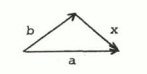
\includegraphics[scale=0.5]{figures_mvc/b_plus_x_equals_a}
	\end{center}
\end{exercise}

In this section we have shown that our definition of vector addition satisfies the same properties as ordinary addition of real numbers. That is, the additive structures are exactly the same for vectors as for numbers. \footnote{To state this more formally, they both form an abelian group.} Therefore, any results that hold for numbers also hold for vectors, for exactly the same reasons. For example,

\begin{thm}[Cancellation law]
	If ${\bf a}, {\bf b},$ and ${\bf c}$ are vectors such that ${\bf a}+{\bf b}={\bf a}+{\bf c}$, then ${\bf b}={\bf c}$. 
\end{thm}

\begin{pf}
The proof for real numbers is as follows: let $x,y,z$ be real numbers such that 
\begin{align*}
	x+y=x+z
\end{align*}
Adding $-x$ to both sides of this equation, we have
\begin{align*}
	-x+(x+y)&=-x+(x+z) \\
	(-x+x)+y&=(-x+x)+z \text{ (since $+$ is associative)} \\
	0+y&=0+z \text{ (since $-x$ is the inverse of $x$)} \\
	y&=z \text{ (since $0$ is the additive identity)}
\end{align*}
Since addition of vectors obeys exactly the same properties as addition of real numbers, this same proof holds for vectors simply by drawing arrows over $x,y$ and $z$!
\end{pf}

\subsubsection{Scalar multiplication}
In physics, we observe that an unbalanced force on a body causes an acceleration in the direction of the force. It is also observed that the magnitude of acceleration of different bodies, when subjected to the same force, varies according to their mass. These observations are formalized in Newton's second law of motion
\begin{equation}
	{\bf F}=m{\bf a}.
\end{equation}
On the right side of this equation, we see a new operation: the product of a scalar and a vector. 

\begin{defn}[Scalar multiplication]
Let $\mathbf{v}$ be a vector and $k$ a scalar. The \emph{scalar multiple} of ${\bf v}$ by $k$ is a vector $\mathbf{w}$, defined as follows:
\begin{itemize}
	\item The length of ${\bf w}$ is $|k|$ times the length of ${\bf v}$. If $|k|=0$, then $\mathbf{w}$ is the zero vector.
	\item $\mathbf{w}$ is parallel to $\mathbf{v}$.
	\item If $k>0$, then $\mathbf{w}$ has the same orientation as $\mathbf{v}$. If $k<0$, then $\mathbf{w}$ and $\mathbf{v}$ have opposite orientation.
\end{itemize}
If $\mathbf{w}$ is the scalar multiple of $\mathbf{v}$ by $k$, we write $\mathbf{w}=k\mathbf{v}$. \footnote{Note that scalar multiplication is not a binary operation on $V$, since it does not take two vectors to a vector, but rather a scalar and a vector to a vector. More formally, scalar multiplication is a map $\R \times V \to V$.}
\end{defn}

\begin{example}
The vector $2{\bf v}$ has the same direction as ${\bf v}$ but twice its length, while $-2{\bf v}$ is oppositely directed to ${\bf v}$ and twice its length. 

\begin{figure}[h]
	\begin{center}
	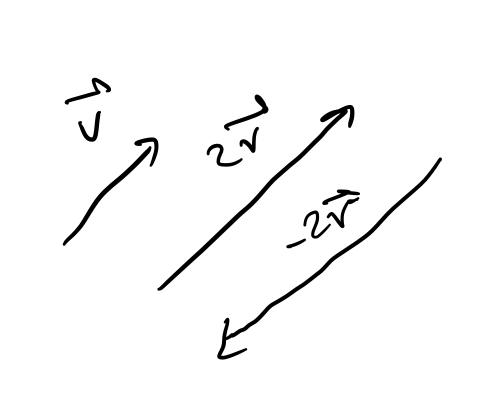
\includegraphics[scale=0.4]{figures_mvc/v2v}
\end{center}
\end{figure}
\end{example}
\newpage
\begin{thm}[Properties of scalar multiplication]\label{thm:properties_of_scalar_multiplication}
For any scalars $c,d$ and vectors ${\bf v}, {\bf w}$, 
	\begin{enumerate}[(i)]
		\item $0{\bf v}={\bf 0}$,
		\item $1{\bf v}={\bf v}$,
		\item $(-1){\bf v}=-{\bf v}$,
		\item $(c+d){\bf v}=c{\bf v}+d{\bf v}$,
		\item $c({\bf v}+{\bf w})=c{\bf v}+c{\bf w}$,
		\item $(dc){\bf v}=c(d{\bf v})$.
	\end{enumerate}
\end{thm}

\begin{pf}
	We will prove pars (i) and (ii) and leave the rest as an exercise. In each case, we need to show that the vector on the left hand side has the same magnitude and direction as the vector on the right hand side. 
	\begin{enumerate}[(i)]
		\item The vector $1\mathbf{v}$ has length $|1|=1$ times the length of $\mathbf{v}$, and therefore has the same length as $\mathbf{v}$. The vector $1\mathbf{v}$ is parallel to $\mathbf{v}$, and since $1>0$ it has the same orientation as $\mathbf{v}$. This shows $1 \mathbf{v}$ has the same magnitude and direction as $\mathbf{v}$, and therefore $1 \mathbf{v}=\mathbf{v}$.
		\item The length of $0\mathbf{v}$ is zero times the length of $\mathbf{v}$, which is zero. Hence, $0\mathbf{v}$ is the zero vector. 
	\end{enumerate} 
\end{pf}

\begin{exercise}
Prove parts (iii)-(vi) of Theorem \ref{thm:properties_of_scalar_multiplication}.	
\end{exercise}

The diligent reader who has worked through the exercises in this section has most likely found many of them to be quite tedious. While the geometric picture of vectors we have developed in this section will be essential for visualization purposes, it is indeed far from optimal for practical computations. This situation will be rectified in the next section by introducing Cartesian coordinate systems in which to describe vectors. \footnote{As should be familiar from freshman geometry, a coordinate system is called Cartesian (or rectangular) if its coordinate axes are all mutually perpendicular.} As we will see, all properties we deduced geometrically in this section will be seen to hold as simple consequences of the properties of real numbers. Despite this simplification of computations, it is important to remember that vectors are geometrical objects whose properties (length and magnitude) do not depend on any particular coordinate system which we may use to describe them.

\subsection{Vectors in coordinate systems}\label{sec:coords}
Let us now describe vectors with respect to a Cartesian coordinate system.

\subsubsection{Vectors in one dimension}
A one-dimensional Cartesian coordinate system is provided by the real number line. Consider a nonzero vector inside the real line; that is, an arrow originating at some point $x_1$ and terminating at a distinct point $x_2$. \footnote{The zero vector has length zero and is therefore just a point.} This vector can point in only one of two directions: either left or right, depending on whether $x_2<x_1$, or $x_1<x_2$, respectively.  Since the location of the vector does not matter, we are free to consider the vector to have initial point at the origin. In this case, the vector originates at the origin, and terminates at some point $x$. The length of the vector is then $|x|$, and its orientation is determined by the sign of $x$, which we denote by $\sgn(x)$, which can be written as $\sgn(x)=\frac{x}{|x|}$. 
\begin{exercise}
	Prove that 
\begin{align*}
	\frac{x}{|x|}=\begin{cases}
		+1, &\text{ if } x>0, \\
		-1, &\text{ if } x<0. \\
	\end{cases}
\end{align*}
\end{exercise}

If we have two such vectors terminating at $x_1$ and $x_2$, respectively, then these vectors are equal if and only if $|x_1|=|x_2|$ and $\sgn(x_1)=\sgn(x_2)$. Since for any $x \neq 0$, we can write
\begin{align*}
	x&=\frac{x}{|x|}|x|\\
	&=\sgn(x)|x|,
\end{align*} 
these vectors are equal if and only if $x_1=x_2$. This shows that there is a 1-1 correspondence between vectors in one-dimension and real numbers, with the correspondence given by
\begin{align*}
	x \leftrightarrow \mathbf{x}=(\sgn(x),|x|).
\end{align*}
We see that there is no essential difference between vectors in one dimension and scalars.

\subsubsection{Vectors in two dimensions}
A two-dimensional Cartesian coordinate system is given by $\R^2=\{(x,y) \mid x,y \in \R\}$. Each point $(x,y) \in \R^2$ specifies the coordinates of a point in a plane. Again, we are free to parallel translate all vectors so that their initial point is at the origin. If the terminal point of such a vector $\mathbf{x}$ is $(x,y)$, then the magnitude of $\mathbf{x}$, which we denote by $||\mathbf{x}||$, \footnote{We use double bars to denote the magnitude of a vector to distinguish this from the absolute value of a real number. Note that, when $\mathbf{x}$ is one dimensional, then $||\mathbf{x}||=\sqrt{x^2}=|x|$.} is given by the Pythagorean theorem 
\begin{align*}
	||\mathbf{x}||=\sqrt{x^2+y^2}.
\end{align*}
We specify the direction of this vector by giving the angle $\theta$ with respect to the positive $x$-axis, which is given by
\begin{align*}
	\theta=\tan^{-1}\left(\frac{y}{x}\right).
\end{align*}
where $\theta \in [0,2\pi)$. Note that this is just the usual change of coordinates from Cartesian to polar coordinates. Since two vectors are equal if and only if $||\mathbf{x_1}||=||\mathbf{x_2}||$ and $\theta_1=\theta_2$, inverting the formulas above
\begin{align*}
	x&=||\mathbf{x}||\cos \theta, \\
	y&=||\mathbf{x}||\sin \theta,
\end{align*}
shows that $(||\mathbf{x}_1||,\theta_1)=(||\mathbf{x}_2||,\theta_2)$ implies $(x_1,y_1)=(x_2,y_2)$. Thus, two-dimensional vectors are in 1-1 correspondence with points in $\R^2$. The coordinates of the end point of the vector are called the \emph{components} of the vector. We will write a two-dimensional vector $\mathbf{v}$ in terms of its components by writing $\mathbf{v}=(v_1,v_2)$. As we have just seen, this expression for $\mathbf{v}$ in terms of its coordinates is unique.

\subsubsection{Vectors is three dimensions}
A three-dimensional Cartesian coordinate system is shown below. 
\begin{center}
	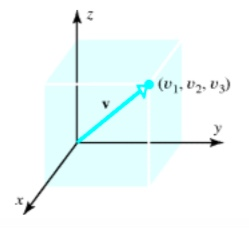
\includegraphics[scale=0.5]{figures_mvc/components}
\end{center}
The coordinate axes are labeled $x,y,$ and $z$, and are arranged such that if you take your right hand and curl your fingers from the positive $x$-axis toward the positive $y$-axis, your thumb points along the positive $z$-axis. Such a coordinate system is called \emph{right-handed}. Again, we find the set of all vectors in three dimensions is in 1-1 correspondence with the set $\R^3=\{(x,y,z) \mid x,y,z \in \R\}$. If $\varphi$ is the angle the vector makes with the positive $z$-axis and $\theta$ is the angle the projection of the vector onto the xy-plane makes with the positive $x$-axis (i.e., it is the usual polar angle in the plane), then the direction of a vector $\mathbf{x}$ is specified by the two angles $(\varphi,\theta)$, where we take $\varphi \in [0,\pi], \theta \in [0,2\pi)$. A little trigonometry shows that the correspondence between $(||\mathbf{x}||,(\varphi,\theta))$ and $(x,y,z)$ is given by
\begin{align}\label{eq:x_spher}
	x&=||\mathbf{x}||\sin \varphi \cos \theta, \\ \label{eq:y_spher}
	y&=||\mathbf{x}||\sin \varphi \sin \theta, \\ \label{eq:z_spher}
	z&=||\mathbf{x}||\cos \varphi. \\
\end{align}
\begin{figure}[h]
\begin{center}
	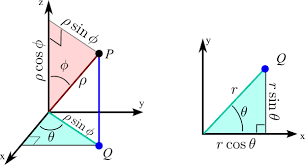
\includegraphics[scale=0.8]{figures_mvc/speric_coor}
\end{center}
\end{figure}
\begin{exercise}
Work out these formulas from the diagram.	
\end{exercise}


As in two-dimensions, we write a three-dimensional vector $\mathbf{v}$ in terms of its components as $\mathbf{v}=(v_1,v_2,v_3)$, and this expression is unique. From the formulas \eqref{eq:x_spher}-\eqref{eq:z_spher}, we see that the length of a vector $\mathbf{v}$ is given by an obvious generalization of the Pythagorean formula
\begin{equation}\label{eq:norm}
	||\mathbf{v}||=\sqrt{v_1^2+v_2^2+v_3^2}.
\end{equation}

\begin{exercise}
	Use the formulas \eqref{eq:x_spher}-\eqref{eq:z_spher} above to prove this.
\end{exercise}


\subsubsection{Vector arithmetic in coordinates}
We now derive the rule for vector addition in terms of components. Given vectors $\mathbf{v}$ and $\mathbf{w}$, we wish to find the components of $\mathbf{v}+\mathbf{w}$. According to the tip-to-tail rule, the $\mathbf{v}+\mathbf{w}$ is given by translating the vector $\mathbf{w}$ so that its initial point coincides with the terminal point of $\mathbf{v}$. This translation moves the $x$-coordinate of $\mathbf{w}$ by $v_1$ units in the $x$-direction, the $y$-coordinate by $v_2$ units in the $y$-direction, and the $z$-coordinate by $v_3$ units in the $z$-direction. That is, 
\begin{align*}
	(w_1,w_2,w_2) \mapsto (v_1+w_1,v_2+w_2,v_3+w_3)
\end{align*}
Thus, the coordinates of the endpoint of $\mathbf{v}+\mathbf{w}$ are given by
\begin{align*}
	\mathbf{v}+\mathbf{w}=(v_1+w_1,v_2+w_2,v_3+w_3).
\end{align*}
\begin{defn}[Vector addition in components]\label{def:vector_addition}
	In terms of components, the rule for vector addition is given by:
\begin{enumerate}[(i)]
	\item Vectors in one-dimension:
	\begin{align*}
		(v_1)+(w_1)=(v_1+w_1)
	\end{align*}
	\item Vectors in two-dimensions:
	\begin{align*}
		(v_1,v_2)+(w_1,w_2)=(v_1+w_1,v_2+w_2).
	\end{align*}
	\item Vectors in three-dimensions:
	\begin{align*}
		(v_1,v_2,v_3)+(w_1,w_2,w_3)=(v_1+w_1,v_2+w_2,v_3+w_3).
	\end{align*}
\end{enumerate}
\end{defn}

This formula is illustrated in the diagram on the left in Figure \ref{fig:vector_operations}.

\begin{example}
Let $\mathbf{v}=(1,2,3)$ and $\mathbf{w}=(-3,1,7)$. Then 
\begin{align*}
	\mathbf{v}+\mathbf{w}=(-2,3,10).
\end{align*}	
\end{example}


\begin{exercise}
	\begin{enumerate}[(a)]
		\item Use the formula in Definition \ref{def:vector_addition} to show that vector addition is commutative.
		\item Use the formula in Definition \ref{def:vector_addition} to show that vector addition is associative.
		\item What are the components of the zero vector?
		\item Given a vector $\mathbf{v}=(v_1,v_2,v_3)$, what are the components of $-\mathbf{v}$ (the additive inverse of $\mathbf{v}$)?
	\end{enumerate}
\end{exercise}
\newpage
\begin{prop}\label{prop:scalar_multiple_formula}
If $\mathbf{v}=(v_1,v_2,v_3)$ is a vector and $k$ a scalar, then the components of the scalar multiple $k\mathbf{v}$ of $\mathbf{v}$ by $k$ are given by
\begin{enumerate}[(i)]
	\item Vectors in one dimension:
	\begin{align*}
		k(v_1)&=(kv_1) \\
	\end{align*}
	\item Vectors in two dimensions:
	\begin{align*}
		k(v_1,v_2)&=(kv_1,kv_2) \\
	\end{align*}
	\item Vectors in three dimensions:
	\begin{align*}
		k(v_1,v_2,v_3)&=(kv_1,kv_2,kv_3)
	\end{align*}
\end{enumerate}	
\end{prop}

\begin{exercise}
	\begin{enumerate}[(a)]
		\item Prove these formulas for vectors in one and two dimensions.
		\item Use this formula to prove that $||k\mathbf{v}||=|k| \cdot ||\mathbf{v}||$ for vectors in three dimensions.
		\item Show that if $k>0$, then $k\mathbf{v}$ has the same direction as $\mathbf{v}$. \footnote{This formula still holds if $k<0$, but checking this case involves some care since $\varphi$ must stay in the range $[0,\pi)$ and $\theta$ in $[0,2\pi)$.} 
	\end{enumerate}
\end{exercise}

\begin{example}
Let $\mathbf{v}=(1,2,3)$ and $k=3$. Then
\begin{align*}
	k\mathbf{v}=(3,6,9).
\end{align*}	
\end{example}

The formula in \eqref{prop:scalar_multiple_formula} is illustrated in the diagram on the right in Figure \ref{fig:vector_operations}.


\begin{exercise}
Use the formula in Proposition \eqref{prop:scalar_multiple_formula} to prove Theorem \eqref{thm:properties_of_scalar_multiplication}.	
\end{exercise}

\begin{figure}\label{fig:vector_operations}
	\begin{center}
	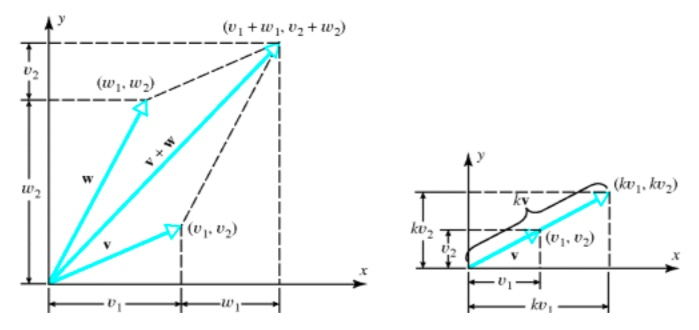
\includegraphics[scale=0.5]{figures_mvc/vector_operations}
\end{center}	
\caption{Vector operations in components.}
\end{figure}

\begin{exercise}
Prove that if $\mathbf{v}=(v_1,v_2,v_3)$ and $\mathbf{w}=(w_1,w_2,w_3)$, then
\begin{align*}
	\mathbf{v}-\mathbf{w}=(v_1-w_1,v_2-w_2,v_3-w_3).
\end{align*}	
\end{exercise}

 The distance between two points $(v_1,v_2,v_3)$ and $(w_1,w_2,w_3)$ in $\mathbb{R}^3$ is therefore given by
\begin{align*}
	||\mathbf{v}-\mathbf{w}||=\sqrt{(v_1-w_1)^2+(v_2-w_2)^2+(v_3-w_3)^2}.
\end{align*}

\begin{example}
\begin{enumerate}[(a)]
	\item Find the components of the vector $\overrightarrow{P_1P_2}$ with initial point $P_1(2,-1,4)$ and terminal point $P_2(7,5,-8)$.
	\item Find the distance between $P_1(2,-1,4)$ and $P_2(7,5,-8)$.
\end{enumerate}	
\end{example}

{\color{red} \flushleft {\bf Solution:} 
\begin{enumerate}[(a)]
	\item The components of $\overrightarrow{P_1P_2}$ are given by
	\begin{align*}
		\overrightarrow{P_1P_2}=(7-2,5-(-1),-8-4)=(5,6,-12)
	\end{align*}
	\item The distance between $P_1$ and $P_2$ is 
	\begin{align*}
		||\overrightarrow{P_1P_2}||=\sqrt{5^2+6^2+(-12)^2}=\sqrt{205}.
	\end{align*}
\end{enumerate}}

\subsubsection{Unit vectors}
\begin{defn}[Unit vector]
	A \emph{unit vector} is a vector of unit length. That is, a vector ${\bf v}$ such that $||{\bf v}||=1$.
\end{defn}

\begin{prop}[Normalizing a vector]
	If ${\bf v}\neq 0$, then ${\bf v}/||{\bf v}||$ is a unit vector in the direction of ${\bf v}$. The unit vector ${\bf v}/||{\bf v}||$ is often denoted ${\bf \hat{v}}$ and the process of forming ${\bf \hat{v}}$ from ${\bf v}$ is called \ti{normalizing} ${\bf v}$.
\end{prop}

\begin{pf}
Since ${\bf v}\neq 0$, $||{\bf v}|| \neq 0$, so we can multiply ${\bf v}$ by $1/||{\bf v}||$. Computing the length of $||\frac{{\bf v}}{||{\bf v}||}||$, we see that 
\begin{align*}
	||\frac{{\bf v}}{||{\bf v}||}||&=\frac{||{\bf v}||}{||{\bf v}||}=1,
\end{align*} 
hence ${\bf v}/||{\bf v}||$ is a unit vector. Since ${\bf v}/||{\bf v}||$ is a scalar multiple of ${\bf v}$ (by $k=1/||{\bf v}||$) it is parallel to ${\bf v}$, and since $k>0$, ${\bf v}/||{\bf v}||$ has the same orientation as $\mathbf{v}$.
\end{pf}

\begin{example}
	We can express any nonzero vector ${\bf v}$ as a product of its magnitude and direction by means of the formula \footnote{Note that this is a generalization of the formula $x=|x|\frac{x}{|x|}$ for a nonzero real number $x$.}
	\begin{align*}
		{\bf v}=||{\bf v}||\frac{{\bf v}}{||{\bf v}||}.
	\end{align*}
	For example, taking ${\bf v}=(1,-2,3)$,
	\begin{align*}
		||{\bf v}||=\sqrt{1^2+(-2)^2+3^2}=\sqrt{14}
	\end{align*}
	and thus
	\begin{align*}
		{\bf v}=\sqrt{14}(\frac{1}{\sqrt{14}},\frac{-2}{\sqrt{14}},\frac{3}{\sqrt{14}}).
	\end{align*}
\end{example}


\begin{defn}[Standard unit vectors]
	 The \ti{standard unit vectors} for $\mathbb{R}^3$ are the vectors
	\begin{align*}
		{\bf i}&=(1,0,0), \\
		{\bf j}&=(0,1,0), \\
		{\bf k}&=(0,0,1). \\
	\end{align*}
These vectors are unit vectors pointing along the $x$-, $y$-, and $z$-axes, respectively. \footnote{The standard unit vectors $({\bf i},{\bf j},{\bf k})$ are also commonly denoted as $({\bf e}_1, {\bf e}_2, {\bf e}_3)$ or $({\bf \hat{x}}, {\bf \hat{y}}, {\bf \hat{z}})$.}	
\end{defn}
Using the standard unit vectors, we may write the vector ${\bf v}=(v_1,v_2,v_3)$ as $${\bf v}=v_1{\bf i}+v_2{\bf j}+v_3{\bf k}.$$
A sum of this form is said to be a \emph{linear combination} of the vectors ${\bf i},{\bf j},{\bf k}$. You should be comfortable working with both expressions for a vector $\mathbf{v}$ in terms of its components.

\begin{example}
Find a unit vector in the direction of the vector from $P_1(1,0,1)$ to $P_2(3,2,0)$.
\end{example}

{\color{red} \flushleft {\bf Solution:}
We find $\overrightarrow{P_1P_2}$ and normalize:
\begin{align*}
	\overrightarrow{P_1P_2}&=(3-1,2-0,0-1)=(2,2,-1), \\
	||\overrightarrow{P_1P_2}||&=\sqrt{2^2+2^2+(-1)^2}=3, \\
\end{align*}
and therefore the desired unit vector is given by
\begin{align*}
	\frac{\overrightarrow{P_1P_2}}{||\overrightarrow{P_1P_2}||}=(\frac{2}{3},\frac{2}{3},-\frac{1}{3}).
\end{align*}}

\begin{example}
Find a vector 6 units long in the direction of ${\bf v}=(2,2,-1)$.	
\end{example}

{\color{red} \flushleft {\bf Solution:}
The vector we want is 
\begin{align*}
6\frac{{\bf v}}{||{\bf v}||}=6\frac{(2,2,-1)}{\sqrt{2^2+2^2+(-1^2)}}=6\frac{(2,2,-1)}{3}=(4,4,-2).	
\end{align*}
}

\subsubsection{The dot product}
Two nonzero vectors ${\bf u}$ and ${\bf v}$ positioned so that their initial points coincide determine an angle $\theta \in [0,\pi]$, which is the angle between the two vectors.
\begin{center}
	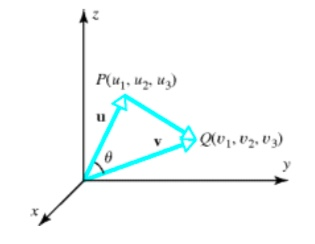
\includegraphics[scale=0.5]{figures_mvc/angle_uv}
\end{center}
Note that the information about $\theta$ is encoded in ${\bf u}-{\bf v}$, since if we fix the magnitudes of ${\bf u}$ and ${\bf v}$ and open the angle, then ${\bf u}-{\bf v}$ will also change. The fundamental relation satisfied by ${\bf u}, {\bf v}$ and $\theta$ is the law of cosines, which says that if ${\bf w}={\bf u}-{\bf v}$, then
\begin{equation}\label{eq:law_of_cosines}
	||{\bf w}||^2=||{\bf u}||^2+||{\bf v}||^2-2||{\bf u}|| \ ||{\bf v}||\cos \theta. 
\end{equation}
Let us make the following definition.
\begin{defn}[Dot product]
	The \emph{dot product} of two nonzero vectors ${\bf u}$ and ${\bf v}$ is defined by
	\begin{equation}\label{eq:dot_product_def}
		{\bf u}\cdot {\bf v}=||{\bf u}|| \ ||{\bf v}||\cos\theta.
	\end{equation} 
\end{defn}
The angle between two vectors ${\bf u}$ and ${\bf v}$ is then given in terms of their dot product by
\begin{equation}\label{eq:angle_uv}
	\theta=\cos^{-1}\left(\frac{{\bf u}\cdot {\bf v}}{||{\bf u}|| \ ||{\bf v}||}\right),
\end{equation}	
and we see that
\begin{itemize}
	\item $\theta$ is acute if ${\bf u} \cdot {\bf v} > 0$.
	\item $\theta$ is obtuse if ${\bf u} \cdot {\bf v} < 0$.
	\item $\theta$ is right if ${\bf u} \cdot {\bf v} = 0$.
\end{itemize}

Since the dot product takes as input two vectors and returns a scalar, it is also called the \emph{scalar product}. Note that from Eq. \eqref{eq:law_of_cosines}, we can write ${\bf u}\cdot {\bf v}$ in terms of magnitudes only, as 
\begin{equation}\label{eq:dot_product_magnitudes}
	{\bf u}\cdot {\bf v}=\frac{||{\bf u}||^2+||{\bf v}||^2-||{\bf u}-{\bf v}||^2}{2}.
\end{equation}
Note that, unlike \eqref{eq:dot_product_def}, the right hand side of \eqref{eq:dot_product_magnitudes} is defined if either $\mathbf{u}=\mathbf{0}$ or $\mathbf{v}=\mathbf{0}$, in which case $\mathbf{u}\cdot \mathbf{v}=0$. Thus, we define the dot product of any vector with the zero vector to be zero:
\begin{align}
	\mathbf{v}\cdot \mathbf{0}=0
\end{align}
for every vector $\mathbf{v}$.

Since \eqref{eq:dot_product_magnitudes} involves only lengths of segments and angles between segments, it holds in \emph{all} coordinate systems. However, it takes a particularly simple form in Cartesian coordinates. Writing out the norm of each vector in terms of its components gives

\begin{align}\label{eq:dot_mess}
	{\bf u}\cdot {\bf v}&=\frac{u_1^2+u_2^2+u_3^2+v_1^2+v_2^2+v_3^2-(u_1-v_1)^2-(u_2-v_2)^2-(u_3-v_3)^2}{2}
\end{align}
Expanding the binomials and cancelling like terms, we find
\begin{equation}\label{eq:dot_simplified}
	{\bf u}\cdot {\bf v}=u_1v_1+u_2v_2+u_3v_3.
\end{equation}

\begin{exercise} 
Simplify equation \eqref{eq:dot_mess} to obtain \eqref{eq:dot_simplified}. 	
\end{exercise}


\begin{example}
Compute the angle between the vectors ${\bf u}=(0,0,3)$ and ${\bf v}=(\sqrt{2},0,\sqrt{2})$.	
\end{example}

{\color{red} \flushleft {\bf Solution:} The angle between these vectors is
\begin{align*}
	\theta=\cos^{-1}\left(\frac{0(\sqrt{2}+0(0)+3(\sqrt{2}))}{3(2)}\right)=\cos^{-1}\left(\frac{1}{\sqrt{2}}\right)=\frac{\pi}{4}.
\end{align*}}

\begin{example}
	Find the angle between a diagonal of a cube and one of its edges.
\end{example}

{\color{red} \flushleft {\bf Solution:}
Let $s$ be the length of an edge and place the cube in the first octant so that one vertex is at the origin and two edges are along the $x$- and $y$-axes.
\begin{center}
	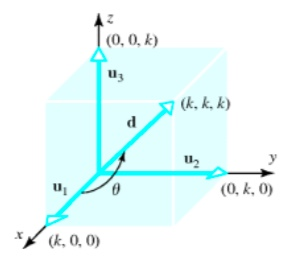
\includegraphics[scale=0.5]{figures_mvc/cube_coordinates}
\end{center}
If we let ${\bf u}_1=(s,0,0), {\bf u}_1=(0,s,0)$, and ${\bf u}_3=(0,0,s)$, then the vector
\begin{align*}
	{\bf d}=(s,s,s)={\bf u}_1+{\bf u}_2+{\bf u}_3
\end{align*}
is a diagonal of the cube. The angle between ${\bf d}$ and ${\bf u}_1$ is 
\begin{align*}
	\theta &=\cos^{-1}\left(\frac{{\bf u}_1 \cdot {\bf d}}{||{\bf u}_1 || \ || {\bf d}||}\right) \\
	&=\cos^{-1}\left(\frac{s^2}{(s)(\sqrt{3s^2})}\right)  \\
	&=\cos^{-1}\left(\frac{1}{\sqrt{3}}\right) \\
	&\approx 54.74^\circ.
\end{align*}
}
\newpage
\begin{prop}[Properties of the dot product]\label{prop:dot}
	Let ${\bf a}, {\bf b}, {\bf c}, {\bf d}$ be vectors and $k$ any scalar. Then 
	\begin{enumerate}[(1)]
		\item ${\bf a}\cdot {\bf b}={\bf b} \cdot {\bf a}$
		\item $(k {\bf a})\cdot {\bf b}={\bf a}\cdot (k{\bf b})=k({\bf a}\cdot {\bf b})$
		\item ${\bf a}\cdot ({\bf b}+{\bf c})={\bf a}\cdot {\bf b}+{\bf a}\cdot {\bf c}$
		\item $({\bf a}+{\bf b})\cdot {\bf a}={\bf a}\cdot {\bf c}+{\bf b}\cdot {\bf c}$
		\item $({\bf a}+{\bf b})\cdot ({\bf c}+{\bf d})={\bf a}\cdot {\bf c}+{\bf a}\cdot {\bf d}+{\bf b}\cdot {\bf c}+{\bf b}\cdot {\bf d}$
		\item ${\bf a} \cdot {\bf a}=||{\bf a}||^2$
	\end{enumerate}
\end{prop}

\begin{pf}
Each of these can be proved by writing out the vectors in components and using  \eqref{eq:dot_simplified}. For example, to prove (1)
\begin{align*}
	{\bf a}\cdot {\bf b}&=a_1b_1+a_2b_2+a_3b_3 \\
	&=b_1a_1+b_2a_2+b_3a_3 \\
	&={\bf b}\cdot {\bf a}
\end{align*}
Properties (2)-(6) are proved similarly. Note that (5) follows from (3) and (4), but is included for emphasis since it is used frequently. 	
\end{pf}

\begin{exercise}
Prove properties (2)-(6) in Proposition \ref{prop:dot}.	
\end{exercise}


Note, however, the differences between the dot product and ordinary multiplication. For instance, one might ask, ``Is the dot product associative?". This question doesn't even make sense for the dot product, as expressions such as ${\bf a}\cdot ({\bf b}\cdot {\bf c})$ are not defined, since ${\bf a}$ is a vector and $({\bf b}\cdot {\bf c})$ is a scalar, and one can only form the dot product between two vectors. Thus, even though we found that the additive structure on the set of vectors was exactly the same as that of the real numbers, the multiplicative structure induced by the dot product is very different from that of the real numbers. 

\subsubsection{Orthogonal vectors}
While writing vectors in component form has the advantage of facilitating many computations, this form seems to obscure geometric relations between vectors.
For instance, the two vectors
\begin{align*}
	{\bf u}&=(3,-2,1) \\
	{\bf v}&=(0,2,4).
\end{align*}
are perpendicular (see Fig. \ref{fig:orthog_vecz} below), but this does not seem obvious from looking at the components of the two vectors. 
\begin{figure}[h]\label{fig:orthog_vecz}
	\begin{center}
		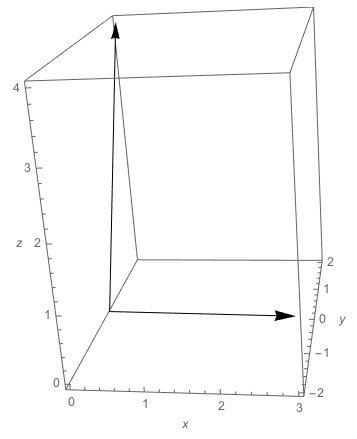
\includegraphics[scale=0.5]{figures_mvc/orthog_vecz}
	\end{center}
	\caption{Orthogonal vectors $\mathbf{u}=(3,-2,1)$ and $\mathbf{v}=(0,2,4)$.}
\end{figure}


We know from trigonometry that right angles are special, so it would be nice to have a way to check if two vectors written in component form are perpendicular. Fortunately, the dot product gives us an easy way to determine this. 
\begin{defn}[Orthogonal vectors]\label{prop:orthogonal_vectors}
	Two nonzero vectors ${\bf a}$ and ${\bf b}$ are said to be \emph{orthogonal} if ${\bf a}\cdot {\bf b}=0$.
\end{defn}
To see the significance of this definition, if ${\bf a}$ and ${\bf b}$ are non-zero then their dot product can be written as
\begin{align*}
	{\bf a}\cdot {\bf b}=||{\bf a}|| \ ||{\bf b}||\cos \theta.
\end{align*}	
Since $||{\bf a}||$ and $||{\bf b}||$ are both greater than zero, ${\bf a}\cdot {\bf b}=0$ if and only if $\theta=\frac{\pi}{2}$, that is, if and only if ${\bf a}$ and ${\bf b}$ are \emph{perpendicular}. Therefore for nonzero vectors being orthogonal (zero dot product) is the same as being perpendicular (intersecting at a right angle). Since $\mathbf{v}\cdot \mathbf{0}=0$ for every vector $\mathbf{v}$, the zero vector is orthogonal to every vector (including itself).

\begin{example}
The two vectors in the example above	
\begin{align*}
	{\bf u}&=(3,-2,1) \\
	{\bf v}&=(0,2,4).
\end{align*}
are orthogonal (and therefore indeed perpendicular) since ${\bf u}\cdot {\bf v}=3(0)-2(2)+1(4)=-4+4=0$.
\end{example}

\begin{defn}[Orthogonal set]
	A set of vectors $\{\mathbf{v}_1,\mathbf{v}_2,\dots,\mathbf{v}_n\}$ is said to be \emph{orthogonal} if $\mathbf{v}_i \cdot \mathbf{v}_j=0$ whenever $i \neq j$.
\end{defn}


\begin{example}
	The standard unit vectors for $\mathbb{R}^3$ form an orthogonal set. One can easily verify that 
	\begin{align*}
		{\bf e}_i \cdot {\bf e_j}=\delta_{ij}
	\end{align*}
where 
\begin{align*}
	\delta_{ij} \equiv \begin{cases}
		1 \text{ if } i=j, \\
		0 \text{ if } i \neq j
	\end{cases}
\end{align*}
is called the \ti{Kronecker delta symbol}. Since ${\bf e}_i \cdot {\bf e_j}=0$ whenever $i \neq j$, the set $\{e_1, e_2, e_3\}$ is indeed orthogonal. 
\end{example}
In the orthogonal set in the previous example, each vector in the set is a unit vector. Such a set has a special name:

\begin{defn}[Orthonormal set]
	An orthogonal set of vectors is said to be an \emph{orthonormal set} if each vector in the set is a unit vector.
\end{defn}


The examples above illustrate another difference between the dot product of two vectors and the ordinary product of two numbers. For two real numbers, if $ab=0$, then either $a=0$ or $b=0$. These examples clearly show that if ${\bf a}\cdot {\bf b}=0$, then it need not be true that either ${\bf a}=0$ or ${\bf b}=0$.
\subsubsection{Projection of a vector}
Let ${\bf a}$ be a nonzero vector, ${\bf \hat{a}}=\frac{{\bf a}}{||{\bf a}||}$ the unit vector obtained by normalizing ${\bf a}$, and ${\bf b}$ another vector. Then Eq. \eqref{eq:dot_product_def} shows that
\begin{align*}
	{\bf \hat{a}}\cdot {\bf b}=\frac{{\bf a}}{||{\bf a}||} \cdot {\bf b}=||{\bf b}||\cos \theta
\end{align*} 
is the component of ${\bf b}$ in the direction of ${\bf a}$. Multiplying by ${\bf \hat{a}}$, we get a vector parallel to ${\bf a}$ whose magnitude is the component of ${\bf b}$ along ${\bf a}$.

\begin{defn}[Vector projection]
	The vector $\text{proj}_{\bf a}{\bf b}\equiv ({\bf \hat{a}}\cdot {\bf b}){\bf \hat{a}}=||{\bf b}||\cos \theta {\bf \hat{a}}$ is called the \ti{projection of ${\bf b}$ onto ${\bf a}$}.
\end{defn}
Geometrically, the projection of ${\bf b}=\overrightarrow{PQ}$ onto ${\bf a}=\overrightarrow{PS}$ is the vector $\overrightarrow{PR}$ determined by connecting a perpendicular segment from $Q$ to the line $PS$. \footnote{Note that by using the definitions of the dot product and the norm of ${\bf a}$, one may produce many equivalent expressions for $\text{proj}_{\bf a}{\bf b}$:
\begin{align*}
	\text{proj}_{\bf a}{\bf b}&=(||{\bf b}||\cos \theta){\bf \hat{a}} \\
	&=({\bf \hat{a}}\cdot {\bf b}){\bf \hat{a}} \\
	&=\left(\frac{{\bf a}\cdot {\bf b}}{||{\bf a}||}\right)\frac{{\bf a}}{||{\bf a}||} \\
	&=\left(\frac{{\bf b}\cdot {\bf a}}{{\bf a}\cdot {\bf a}}\right){\bf a}
\end{align*}
The first of these is perhaps the easiest to remember, as it makes most transparent the relation to elementary right triangle trigonometry.}

\begin{center}
	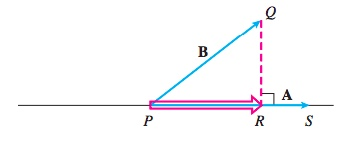
\includegraphics[scale=0.5]{figures_mvc/vector_projection_def}
\end{center}
Physically, if ${\bf b}$ represents a force, then $\text{proj}_{\bf a}{\bf b}$ is the 	``effective" force in the ${\bf a}$ direction; that is, the component of the force along ${\bf a}$.

\begin{center}
	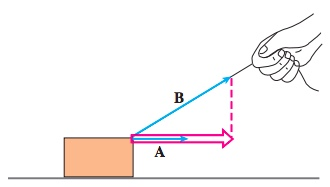
\includegraphics[scale=0.5]{figures_mvc/effective_force_box}
\end{center}	

It is often desirable to express a vector ${\bf b}$ as a sum of two orthogonal vectors. For instance, in mechanics we frequently decompose forces in this way so that we may treat a two-dimensional problem as two one-dimensional problems. We can easily express a vector ${\bf b}$ as such a sum of two vectors, one parallel to some nonzero vector ${\bf a}$ and one orthogonal to ${\bf a}$, in terms of the projection of ${\bf b}$ along ${\bf a}$:
\begin{equation}
\begin{split}
	{\bf b}&={\bf b}_{\parallel}+{\bf b}_{\perp} \\
	&=\text{proj}_{\bf a}{\bf b}+({\bf b}-\text{proj}_{\bf a}{\bf b}).
\end{split}
\end{equation}

\begin{center}
	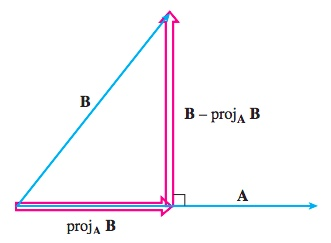
\includegraphics[scale=0.5]{figures_mvc/sum_of_orthogonal_vectors}
\end{center}

\begin{example}
	Express ${\bf b}=2{\bf e}_1+{\bf e}_2-3{\bf e}_3$ as the sum of a vector parallel to ${\bf a}=3{\bf e}_1-{\bf e}_2$ and a vector orthogonal to ${\bf a}$.
\end{example}

{\color{red} \flushleft {\bf Solution:}
Since ${\bf \hat{a}}\equiv \frac{{\bf a}}{||{\bf a}||}=\frac{3{\bf e}_1-{\bf e}_2}{\sqrt{10}}$, we can write ${\bf b}={\bf b}_{\parallel}+{\bf b}_{\perp}$ with  
\begin{align*}
	{\bf b}_{\parallel}&=({\bf \hat{a}}\cdot {\bf b}){\bf {\hat{a}}}=\frac{1}{2}(3{\bf e}_1-{\bf e}_2)=\frac{1}{2}{\bf a} \\
	{\bf b}_{\perp}&={\bf b}-{\bf b}_{\parallel}=\frac{1}{2}{\bf e}_1+\frac{3}{2}{\bf e}_2-3{\bf e}_3.
\end{align*}}

\subsection{Equations of lines and planes}
\subsubsection{Lines in space}
The coordinate systems of analytic geometry allow us to consider geometric objects such as lines and planes in terms of vectors. These geometric ideas will give us valuable intuition later on in the course when we take a more abstract point of view toward vectors.

First let us recall that any two points define a line. Equivalently, we can also determine a line if we know one point on the line and the slope of the line. 

Let us now work in Cartesian coordinates. Suppose $L$ is a line passing through a point $P_0(x_0,y_0,z_0)$ and parallel to a vector ${\bf v}=v_1{\bf e}_1+v_2{\bf e}_2+v_3{\bf e}_3$. Now let $P(x,y,z)$ be any point in space. In which case will $P(x,y,z)$ to be on the line? This will be the case if and only if the vector $\overrightarrow{P_0P}$ is parallel to ${\bf v}$, that is, if $\overrightarrow{P_0P}$ is a scalar multiple of ${\bf v}$. Therefore,
\begin{defn}[Vector equation for a line]
	The line through $P_0(x_0,y_0,z_0)$ and parallel of ${\bf v}$ is the set of all points $P(x,y,z)$ such that $\overrightarrow{P_0P}=t{\bf v}$, with $-\infty < t < \infty$. This equation is called the \ti{vector equation} of the line.
\end{defn}
In terms of Cartesian coordinates, the vector equation for the line becomes
\begin{align*}
	(x-x_0){\bf e}_1+(y-y_0){\bf e}_2+(z-z_0){\bf e}_3&=t(v_1{\bf e}_1+v_2{\bf e}_2+v_3{\bf e}_3) \\
	&=tv_1{\bf e}_1+tv_2{\bf e}_2+tv_3{\bf e}_3
\end{align*}
which implies
\begin{align*}
	(x-x_0-tv_1){\bf e}_1+(y-y_0-tv_2){\bf e}_2+(z-z_0-tv_3){\bf e}_3={\bf 0}
\end{align*}
and hence
\begin{equation}\label{eq:parametric_equations_line}
	x=x_0+tv_1, \hspace{0.25cm} y=y_0+tv_2, \hspace{0.25cm} z=z_0+tv_3.
\end{equation}
Thus, the vector equation of the line is equivalent to the three scalar equations in Eq. \eqref{eq:parametric_equations_line}, each of which is the usual equation for a line with slope $v_i$ in one variable $t$.

\begin{defn}[Parametric equations for a line]
	The standard parametrization of the line through $P_0(x_0,y_0,z_0)$ and parallel to ${\bf v}=v_1{\bf e}_1+v_2{\bf e}_2+v_3{\bf e}_3$ is given by
	\begin{align*}
		x=x_0+tv_1, \hspace{0.25cm} y=y_0+tv_2, \hspace{0.25cm} z=z_0+tv_3.
	\end{align*}
	These equations are called the (standard) \ti{parametric equations} for the line.
\end{defn}

\begin{example}
Find the parametric equations for the line through $(-2,0,4)$ and parallel to ${\bf v}=2{\bf e}_1+4{\bf e}_2-2{\bf e}_3$.	
\end{example}

{\color{red} \flushleft {\bf Solution:}
Plugging into Eq. \eqref{eq:parametric_equations_line} gives
\begin{align*}
	x=-2+2t, \hspace{0.25cm} y=4t, \hspace{0.25cm} z=4-2t.
\end{align*}}
\begin{center}
	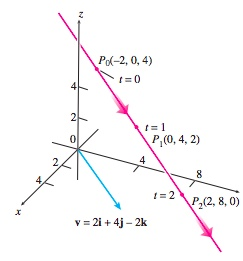
\includegraphics[scale=0.5]{figures_mvc/parametrized_line_example_1}
\end{center}

\begin{example}
	Find parametric equations for the line through $P(-3,2,-3)$ and $Q(1,-1,4)$.
\end{example}

{\color{red} \flushleft {\bf Solution:}
The vector from $P$ to $Q$ is 
\begin{align*}
	\overrightarrow{PQ}&=(1-(-3), -1-2, 4-(-3)) \\
	&=(4,-3,7).
\end{align*}
We take this vector to be our ``${\bf v}$". The point $P_0$ could be either $P$ or $Q$. Arbitrarily choosing it to be $Q$, Eq. \eqref{eq:parametric_equations_line} gives
\begin{align*}
	x=1+4t, \hspace{0.25cm} y=-1-3t, \hspace{0.25cm} z=4+7t.
\end{align*}}

\begin{example}
Parametrize the line segment joining the points $P(-3,2,-3)$ and $Q(1,-1,4)$.	
\end{example}
{\color{red} \flushleft {\bf Solution:}
We have seen in the previous exercise that the  parametric equations 
\begin{align*}
	x=1+4t, \hspace{0.25cm} y=-1-3t, \hspace{0.25cm} z=4+7t.
\end{align*}
describe an infinite line containing $P$ and $Q$ when we take $-\infty < t < \infty$. To describe the line segment joining $P$ and $Q$, we simply restrict the domain of $t$. We see that the line passes through $P$ at $t=-1$ and $Q=0$. So the line segment joining $P$ and $Q$ is given by 

\begin{align*}
	x=1+4t, \hspace{0.25cm} y=-1-3t, \hspace{0.25cm} z=4+7t.
\end{align*}

with $-1 < t < 0$.}

In $\mathbb{R}^2$, there is a unique normal direction to a given line. Let $\mathbf{n}=(n_1,n_2)$ be a normal vector to a line in $\mathbb{R}^2$ and $P_0(x_0,y_0)$ any point on the line. If $Q(x,y)$ is any other point on the line, then we must have
\begin{align*}
	\overrightarrow{P_0Q}\cdot \mathbf{n}=0.
\end{align*}
Since $\overrightarrow{P_0Q}=(x-x_0,y-y_0)$, 
\begin{align*}
	\overrightarrow{P_0Q}\cdot \mathbf{n}&=n_1(x-x_0)+n_2(y-y_0)=0
\end{align*}
or
\begin{align}\label{eq:point_normal_equation_for_line}
	n_1x+n_2y=c
\end{align}
where $c=n_1x_0+n_2y_0$. Equation \eqref{eq:point_normal_equation_for_line} is called the \emph{point normal} equation of the line.

\subsubsection{Planes in space}
Similar to a line in $\mathbf{R}^2$, a plane in $\mathbb{R}^3$ has a unique normal direction. We will now derive a point normal equation for a given plane. Let $\mathbf{n}=(n_1,n_2,n_3)$ be a normal vector to the plane. Given a point $P_0(x_0,y_0,z_0)$ on the plane and a vector ${\bf n}$ normal to the plane, what is the condition for an arbitrary point in space $P(x,y,z)$ to lie on the plane? If $P$ lies in the plane, the $\overrightarrow{P_0P}$ is a vector lying in the plane. Then, since ${\bf n}$ is normal to the plane, we must have that ${\bf n} \cdot \overrightarrow{P_0P}=0$.

\begin{center}
	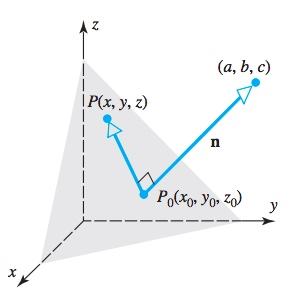
\includegraphics[scale=0.5]{figures_mvc/vector_equation_of_a_plane}
\end{center}
Expanding the dot product in terms of components of these vectors, we obtain
	\begin{equation}
		n_1(x-x_0)+n_2(y-y_0)+n_3(z-z_0)=0.
	\end{equation}
or 
	\begin{equation}
		n_1x+n_2y+n_3z=c
	\end{equation}
	where $c=n_1x_0+n_2y_0+n_3z_0$. This is the \emph{point normal} equation of the plane.


\begin{example}
Find an equation for the plane through $P_0(-3,0,7)$ perpendicular to ${\bf n}=(5,2,-1)$.	
\end{example}

{\color{red} \flushleft {\bf Solution:}
The component equation is 
\begin{align*}
	5(x-(-3))+2(y-0)+(-1)(z-7)=0,
\end{align*}
Simplifying, we obtain
\begin{align*}
	5x+15+2y-z+7&=0 \\
	5x+2y-z&=-22.
\end{align*}}

\begin{example}
Find the point where the line 
\begin{align*}
	x=\frac{8}{3}+2t, \hspace{0.25cm} y=2t, \hspace{0.25cm} z=1+t
\end{align*}	
intersects the plane $3x+2y+6z=6$.
\end{example}

{\color{red} \flushleft {\bf Solution:}
The point $(\frac{8}{3}+2t, 2t, 1+t)$ lies in the plane if its coordinates satisfy the equation of the plane; that is, if
\begin{align*}
	3(\frac{8}{3}+2t)+2(-2t)+6(1+t)=6
\end{align*}
This has a solution at $t=-1$, so the point of intersection is 
\begin{align*}
	(x,y,z)\vert_{t=-1}=(\frac{2}{3},2,0).
\end{align*}}

\begin{exercise}
\begin{enumerate}[(a)]
	\item Find a vector parallel to the line of intersection of the planes $3x-6y-2z=15$ and $2x+y-2z=5$.	
	\item Find parametric equations for the line in which these planes intersect.
\end{enumerate}
\end{exercise}

\subsection{Some useful distance formulas}
\begin{thm}[Distance from point to line or plane] \hspace{15cm}
	\begin{enumerate}[(a)]
		\item In $\R^2$, the distance $D$ between the point $P_0(x_0,y_0)$ and the line $ax+by+c=0$ is 
		\begin{align}\label{eq:line_dist_formula}
			D=\frac{|ax_0+by_0+c|}{\sqrt{a^2+b^2}}
		\end{align}
		\item In $\R^3$ the distance $D$ between the point $P_0(x_0,y_0,z_0)$ and the plane $ax+by+cz+d=0$ is 
		\begin{align}\label{eq:plane_dist_formula}
			D=\frac{|ax_0+by_0+cz_0+d|}{\sqrt{a^2+b^2+c^2}}.
		\end{align}
	\end{enumerate}
\end{thm}

\begin{proof} \hspace{15cm}
	\begin{enumerate}[(a)]
		\item Left as an exercise. The steps are virtually identical to the proof in part (b).		
		\item Let $Q(x_1,y_1,z_1)$ be any point in the plane. Translate the normal vector $\mathbf{n}=(a,b,c)$ so that its initial point is at $Q$. 
	\begin{figure}[h]
		\begin{center}
			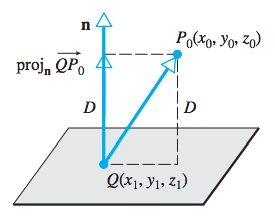
\includegraphics[scale=0.5]{figures_mvc/dist_to_plane_book}
		\end{center}
		\caption{Distance from $P_0$ to the plane.}
	\end{figure} 
		
		The distance $D$ is then the length of the projection $\text{proj}_{\mathbf{n}}\overrightarrow{QP_0}$:
		\begin{align*}
			D&=||\text{proj}_{\mathbf{n}}\overrightarrow{QP_0}|| \\
			&=\left|\left|\frac{\overrightarrow{QP_0}\cdot \mathbf{n}}{\mathbf{n}\cdot \mathbf{n}}\mathbf{n} \right|\right| \\
			&=\left|\frac{\overrightarrow{QP_0}\cdot \mathbf{n}}{\mathbf{n}\cdot \mathbf{n}}\right|||\mathbf{n}|| \\
			&=\frac{|\overrightarrow{QP_0}\cdot \mathbf{n}|}{||\mathbf{n}||^2}||\mathbf{n}|| \\
			&=\frac{|\overrightarrow{QP_0}\cdot \mathbf{n}|}{||\mathbf{n}||}
		\end{align*}
		Now
		\begin{align*}
			\overrightarrow{QP_0}&=(x_0-x_1,y_0-y_1,z_0-z_1), \\
			\overrightarrow{QP_0}\cdot{n}&=a(x_0-x_1)+b(y_0-y_1)+c(z_0-z_1), \\
			||\mathbf{n}||&=\sqrt{a^2+b^2+c^2}.
		\end{align*}
		and therefore
	\begin{align}\label{eq:dist_p_0_to_plane}
			D&=\frac{|\overrightarrow{QP_0}\cdot \mathbf{n}|}{||\mathbf{n}||}\\
			&=\frac{|a(x_0-x_1)+b(y_0-y_1)+c(z_0-z_1)|}{\sqrt{a^2+b^2}}.
		\end{align}
		Since the point $Q(x_1,y_1,z_1)$ lies in the plane, its coordinates satisfy the equation of the plane; thus
		\begin{align*}
			ax_1+by_1+cz_1+d=0
		\end{align*}
		or 
		\begin{align*}
			d=-ax_1-by_1-cz_1.
		\end{align*}
		Substituting this expression into \eqref{eq:dist_p_0_to_plane} yields \eqref{eq:plane_dist_formula}.
	\end{enumerate}
\end{proof}

\begin{example}
By \eqref{eq:plane_dist_formula}, the distance $D$ between the point $P_0(1,-4,-3)$ and the plane $2x-3y+6z=-1$ is
\begin{align*}
	D=\frac{|2(1)+(-3)(-4)+6(-3)+1|}{\sqrt{2^2+(-3)^2+6^2}}=\frac{|-3|}{7}=\frac{3}{7}.
\end{align*}	
\end{example}

The formula \eqref{eq:dist_p_0_to_plane} also allows us to compute the distance between parallel planes.

\begin{example}
The planes
\begin{align*}
	x+2y-2z=3 \hspace{0.25cm} \text{ and } \hspace{0.25cm} 2x+4y-4z=7
\end{align*}	
are parallel since their normal vectors $(1,2,-2)$ and $(2,4,-4)$ are parallel vectors. To find the distance $D$ between the planes, we just select an arbitrary point $P_0$ on one of the planes and then compute its distance to the other plane using \eqref{eq:dist_p_0_to_plane}. By setting $y=z=0$ in the equation $x+2y-2z=3$, we obtain the point $P_0(3,0,0)$ in this plane. The distance between $P_0$ and the plane $2x+4y-4z=7$ is then
\begin{align*}
	D=\frac{|2(3)+4(0)+(-4)(0)-7|}{\sqrt{2^2+4^2+(-4)^2}}=\frac{1}{6}.
\end{align*} 
\end{example}


\section{Systems of linear equations}

\subsection{Basic definitions}
\begin{defn}[Linear equation]\label{def:linear_equation}
	A \ti{linear equation} in the variables $x_1,\cdots, x_n$ is an equation that can be written in the form
\begin{equation}
	a_1 x_1+a_2 x_2+\cdots a_n x_n=b
\end{equation}
where $b$ and the \ti{coefficients} $a_1,\cdots, a_n$ are real or complex numbers	
\end{defn}

\begin{exercise}
\bf Which of the following equations are linear?
\begin{enumerate}[(a)]
	\item $4x_1-5x_2+2=x_1$
	\item $x_2=2\sqrt{x_1}-6$
	\item $2x_1+x_2-x_3=2\sqrt{6}$ 
	\item $4x_1-5x_2=x_1x_2$ 
\end{enumerate}
\end{exercise}

\begin{defn}[System of linear equations]\label{eq:system_of_linear_equations}
	A \ti{system of linear equations} (or a \ti{linear system}) is a collection of one or more linear equations involving the \ti{same} variables $x_1, \cdots, x_n$.	
\end{defn}

\begin{example}
The following is a system of two linear equations in three variables $x_1,x_2,x_3$:
\begin{equation}\label{eq:system}
\begin{split}
	2x_1-x_2+1.5x_3&=8 \\
	x_1  \hspace{1.0cm} - \ 4x_3&=-7
\end{split}
\end{equation}	
\end{example}

\begin{defn}[Solution]\label{def:solution}
	Any $n$-tuple $(s_1,\cdots,s_n)$ of numbers which satisfies \ti{each} equation in a linear system when $s_1,\cdots,s_n$ are substituted for $x_1,\cdots,x_n$ is called a \ti{solution} of the system.
\end{defn}

\begin{example}[Testing a solution]
The 3-tuple $(5,6.5,3)$ is a solution of the system \eqref{eq:system} since
	\begin{equation*}
\begin{split}
	2(5)-6.5+1.5(3)&=8 \\
	5  \hspace{1.0cm} - \ 4(3)&=-7
\end{split}
\end{equation*}	
\end{example}

\begin{defn}[Solution set] \label{def:solution_set}
The set of all solutions is called the \ti{solution set} of the linear system.	
\end{defn}

\begin{defn}[Consistent and inconsistent systems]\label{def:consistent}
If a system of equations has at least one solution it is said to be \ti{consistent}. Otherwise it is said to be \ti{inconsistent}.	
\end{defn}

\begin{exercise}
Is $(3,4,-2)$ a solution of the following linear system?
\begin{align*}
	5x_1-x_2+2x_3 &=7 \\
	-2x_1+6x_2+9x_3&=0 \\
	-7x_1+5x_2-3x_3&=-7
\end{align*} 	
\end{exercise}

\begin{example}[Two linear equations in two unknowns]\label{ex:two_linear_equations_in_two_unknowns}
Consider the most general linear system of two equations in two unknowns
\begin{equation}\label{eq:2_eq_2_var}
	\begin{split}
				A_{11} x_1+A_{12}x_2&=b_1 \\
		A_{21} x_1+A_{22}x_2&=b_2. 
	\end{split}
\end{equation}	
Rewriting each equation in slope-intercept form, \eqref{eq:2_eq_2_var} becomes
\begin{equation}
	\begin{split}
		x_2&=-\frac{A_{11}}{A_{12}}x_1+\frac{b_1}{A_{12}} \\
		x_2&=-\frac{A_{21}}{A_{22}}x_1+\frac{b_2}{A_{22}}
	\end{split}
\end{equation}
Geometrically, each equation describes a line in the Euclidean plane. Since these equations are in the same variables, the two lines lie in the same plane. A solution to the linear system corresponds to a point which lies on \ti{both} lines at the same time, so it is a point of intersection of the two lines. There are therefore three possibilities for the possible solution sets of the linear system \eqref{eq:2_eq_2_var}, depending on the coefficients:
\begin{enumerate}[(1)]
	\item The linear system \eqref{eq:2_eq_2_var} has \emph{no solution} when 
	\begin{align*}
		\frac{A_{11}}{A_{12}}&=\frac{A_{21}}{A_{22}}, \\
		b_1 & \neq b_2,
	\end{align*}
i.e., when the lines are parallel (same slope) but non-overlapping (different y-intercepts).
\begin{center}
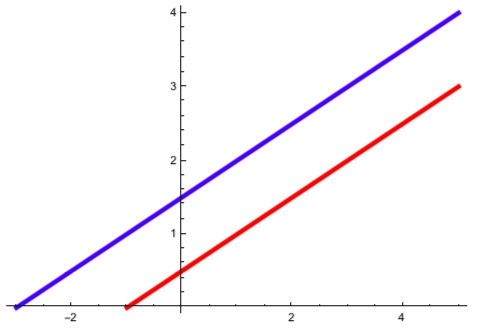
\includegraphics[scale=0.5]{figures_mvc/two_lines_no_soln}
\end{center}

\item The linear system \eqref{eq:2_eq_2_var} has \emph{infinitely many solutions} when 
	\begin{align*}
		\frac{A_{11}}{A_{12}}&=\frac{A_{21}}{A_{22}}, \\
		b_1 & = b_2,
	\end{align*}
	i.e., when the lines are overlapping (both described by exactly the same equation).
	\begin{center}
	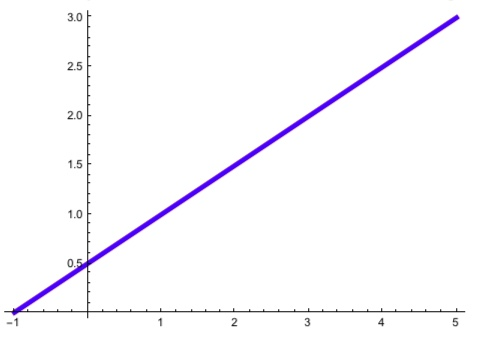
\includegraphics[scale=0.5]{figures_mvc/two_lines_inf_soln}		
	\end{center}

\item The linear system \eqref{eq:2_eq_2_var} has a \emph{unique solution} in all other cases (i.e., when the lines are non-parallel).
\begin{center}
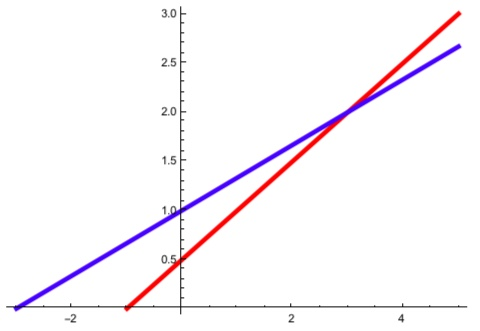
\includegraphics[scale=0.5]{figures_mvc/two_lines_unique_soln}	
\end{center}
\end{enumerate}
\end{example}

In general, we will consider a linear system of $m$ equations in $n$ unknowns:
\begin{equation}\label{eq:m_eq_n_var}
\begin{split}
	A_{11}x_1+A_{12}x_2+\cdots + A_{1n}x_n &=y_1 \\
	A_{21}x_1+A_{22}x_2+\cdots + A_{2n}x_n &=y_2 \\
	\vdots \hspace{1.5cm} \vdots \hspace{2.5cm} \vdots & \hspace{0.5cm}\vdots  \\
	A_{m1}x_1+A_{m2}x_2+\cdots + A_{mn}x_n &=y_m \\
\end{split}	
\end{equation}
where $y_1,\cdots, y_m$ and $A_{ij}, 1 \leq i \leq m, 1 \leq j \leq n$ are given. In \eqref{eq:m_eq_n_var}, we denote the coefficient of $x_j$ in the $i$th equation as $A_{ij}$.


\begin{defn}[Homogeneous and inhomogeneous sytems]\label{def:homogeneous_and_inhomogeneous_sytems}
If $y_1=y_2=\cdots=y_m=0$ in 
\eqref{eq:2_eq_2_var}, the system is said to be \ti{homogeneous}. Otherwise, it is said to be \ti{inhomogeneous}.
\end{defn}
We see later that, for any linear system of $m$ equations and $n$ unknowns, the sizes of the possible solution sets are the same as in Example \ref{ex:two_linear_equations_in_two_unknowns}: any system of linear equations has either no solutions, a unique solutions, or an infinite number of solutions. \footnote{More precisely, by ``infinite number" of solutions here, we mean one solution for each real number. More formally, we say there are $\mathfrak{c}$ solutions, where $\mathfrak{c}=2^{\aleph_0}=|\mathbb{R}|$ is the cardinality of the set of real numbers, called the \ti{continuum}.}
\subsection{Elimination}
A fundamental technique for finding the solutions of a system of linear equations is that of \ti{elimination} of variables. Roughly, this technique involves multiplying the equations in the system by numbers and then adding them together so that some of the variables drop out, leading to a simpler system of equation.
\begin{example}[Solving by elimination]
To illustrate this technique, consider the homogeneous system
	\begin{equation}
		\begin{split}
		2x_1-x_2+x_3&=0 \\
		x_1+3x_2+4x_3&=0.
		\end{split}
	\end{equation} 
Adding $(-2)$ (Eq. 4) +(Eq. 3)  gives $-7x_2-7x_3=0$ or $x_2=-x_3$. Adding
$3$ (Eq. 3) + (Eq. 4) gives $7x_1+7x_3=0$ or $x_1=-x_3$. 
Combining these, we see that this system has an infinite number of solutions. The solution set can be written in \ti{parametric form} as $\{(-t,-t,t): t \in \mathbb{R}\}$ in terms of a single \ti{parameter}, $t$. \footnote{In general, if a system of $m$ equations in $n$ unknowns is consistent but doesn't have a unique solution, then the solution set will depend on up to $n$ parameters. In this case, the solution set will be in 1-1 correspondence with $\mathbb{R}^n$. It is a fact that $|\mathbb{R}^n|=|\mathbb{R}|$ (I won't attempt to explain this here), so the statement that any system of linear equations has $0,1,$ or $\mathfrak{c}$ solutions is true in general. \fixme{Does this mean that we can, in principle, parametrize the solution set in terms of a single parameter? Can this not be done in practice (e.g., is the proof that there exists such a bijection not constructive)? or is this just not useful to do (e.g., that the bijection lacks some desirable properties, such as continuity)? For a historical account, see \cite{cantor_surprised}.}} 
\end{example}
We now begin to formalize the elimination process in order to carry it out in a systematic way and to understand why it works. Consider again the general linear system of $m$ equations in $n$ unknowns in \eqref{eq:m_eq_n_var}. If we select $m$ scalars $c_1,\cdots,c_m$, multiply the $j$th equation by $c_j$ for $j=1,\cdots,m$, and add all of the equations together, we obtain a new linear equation, given by
\begin{equation}\label{eq:linear_combination_of_equations}
	\begin{split}
		(c_1A_{11}+c_2A_{21}+\cdots+c_mA_{m1})x_1+\cdots+(&c_1A_{1n}+c_2A_{21}+\cdots+c_mA_{mn})x_n \\ &= c_1y_1+\cdots +c_m y_m.
	\end{split}
\end{equation}

\begin{defn}[Linear combination]\label{eq:linear_combination_of_equations}
The equation \eqref{eq:linear_combination_of_equations} is said to be a \ti{linear combination} of the equations in \eqref{eq:m_eq_n_var}.
\end{defn}

\begin{prop}[Linear combinations of linear equations preserve solutions]\label{prop:linear_combinations_of_linear_equations_preserve_solutions}
If $(s_1,\cdots,s_n)$ is a solution of the linear system \eqref{eq:m_eq_n_var}, then it is also a solution of \eqref{eq:linear_combination_of_equations}.	
\end{prop}

\begin{pf}
	Substituting $(x_1,\cdots,x_n)=(s_1,\cdots,s_n)$ in \eqref{eq:linear_combination_of_equations} gives
\begin{align*}
	&(c_1A_{11}+c_2A_{21}+\cdots+c_mA_{m1})s_1+\cdots+(c_1A_{1n}+c_2A_{21}+\cdots+c_mA_{mn})s_n  \\
	&=c_1(A_{11}s_1+\cdots + A_{1n}s_n)+\cdots + c_m(A_{m1}s_1+\cdots + A_{mn}s_n) \\
	&= c_1y_1 + \cdots + c_my_m.
\end{align*}
\end{pf}

\ti{Proposition \ref{prop:linear_combinations_of_linear_equations_preserve_solutions} is the fundamental idea of the elimination process}: if we have another system of linear equations
	\begin{equation}\label{eq:another_system}
\begin{split}
	B_{11}x_1+B_{12}x_2+\cdots + A_{1n}x_n &=z_1 \\
	B_{21}x_1+B_{22}x_2+\cdots + B_{2n}x_n &=z_2 \\
	\vdots \hspace{1.5cm} \vdots \hspace{2.5cm} \vdots & \hspace{0.5cm}\vdots  \\
	B_{k1}x_1+B_{k2}x_2+\cdots + B_{kn}x_n &=z_k \\
\end{split}
\end{equation}
in which each of the $k$ equations is a linear combination of the equations in \eqref{eq:m_eq_n_var}, then \emph{every solution of \eqref{eq:m_eq_n_var} is a solution of this new system}. 
Thus, \ti{the elimination process allows us to solve a linear system by forming linear combinations of the given equations to produce an system of equations which has the same solutions, but is easier to solve}. 

However, we need to think carefully about how to do this, as it may happen that some solutions of \eqref{eq:another_system} are not solutions of \eqref{eq:m_eq_n_var}. As a simple example, consider the following two linear systems:
\begin{align}
		x_1-2x_2&=-1 \label{eq:e1}\\
		-x_1+3x_2&=3 \label{eq:e2}
\end{align} 
and 
\begin{align}
		x_1-2x_2&=-1 \label{eq:e3}\\
		-x_1+2x_2&=1 \label{eq:e4}
\end{align}
Using the elimination technique, the former system has a unique solution $(3,2)$ whereas the latter has an infinite number of solutions, which we can parametrize as $\{(2t-1,t):t \in \mathbb{R}\}$. By taking $t=2$, we see that $(3,2)$ is a solution of the second system, but for any solution of the second system with $t \neq 2$ is not a solution of the first.

This can be understood as follows: Both equations in the second system can be written as linear combinations of the equations in the first system, since 
\begin{align*}
	\eqref{eq:e3}&=1\cdot \eqref{eq:e1}+0\cdot \eqref{eq:e2} \\
	\eqref{eq:e4}&=-1\cdot \eqref{eq:e1}+0\cdot \eqref{eq:e2}
\end{align*}
However, the second equation in the first system  cannot be written as a linear combination of the equations in the second system.

\begin{exercise}
Show that 
\begin{align*}
	c_1 \eqref{eq:e3} + c_2 \eqref{eq:e4} = \eqref{eq:e2}
\end{align*}
requires 
\begin{align*}
	c_1-c_2&=-1 \\
	c_1-c_2&=-3,
\end{align*}	
which has no solution.
\end{exercise}

This motivates the following definition:

\begin{defn}[Equivalent linear systems] \label{def: equivalent_linear_systems}
	Two systems of linear equations are said to be \ti{equivalent} if they have the same set of solutions.
\end{defn}

We have just seen that two linear systems might fail to be equivalent if the equations in one system cannot be written as linear combinations of the equations in the other system. We thus have the following proposition:

\begin{prop}[Equivalent linear systems]\label{prop:equivalent_linear_systems}
	Two systems of linear equations are equivalent if each equation in each system is a linear combination of the equations in the other system. 
\end{prop}

\begin{pf}
	The proof follows immediately from Proposition \ref{prop:linear_combinations_of_linear_equations_preserve_solutions}.
\end{pf}

\begin{exercise}
Are the following two systems of linear equations equivalent? If so, express each equation in each system as a linear combination of the equations in the other system.
\begin{align*}
	 x_1-x_2=0 \hspace{1.0cm} 3x_1+x_2&=0 \\
	2x_1+x_2=0 \hspace{1.0cm} x_1+x_2&=0
\end{align*}	
\end{exercise}

If the elimination process is to be effective in finding the solutions of the system \eqref{eq:m_eq_n_var}, then we must see how to form linear combinations of the given equations to produce an \ti{equivalent} system of equations which is easier to solve. In the next section, we will discuss one method of doing this.

\subsection{Matrices}
Given the general system of $m$ linear equations in $n$ unknowns in \eqref{eq:m_eq_n_var}, we wish to form linear combinations of these equations in such a way that we are guaranteed to produce an equivalent system which is easier to solve. In this section, we will formalize this process and make precise the kind of system at which we want to arrive.

	In forming linear combinations of the equations in \eqref{eq:m_eq_n_var}, notice that we are actually only computing with the coefficients $A_{ij}$ and scalars $y_i$. We shall therefore abbreviate the system by
	\begin{equation}
		AX=Y
	\end{equation}
	where 
	\begin{equation}\label{eq:coeff_matrix}
		A=\begin{bmatrix}
			A_{11} \cdots A_{1n} \\
			\vdots \hspace{1.3cm} \vdots \\
			A_{m1} \cdots A_{mn}
		\end{bmatrix}
	\end{equation} 
	\begin{equation}
		X=\begin{bmatrix}
			x_1 \\ \vdots \\ x_n
		\end{bmatrix} \ \text{ and } Y= \begin{bmatrix}
			y_1 \\ \vdots \\ y_m
		\end{bmatrix}
	\end{equation} 
\begin{defn}[Coefficient matrix] \label{def:coefficient_matrix}
	A rectangular array of numbers as in \eqref{eq:coeff_matrix} is called a \ti{matrix}. In \eqref{eq:coeff_matrix}, the matrix $A$ is called the \ti{coefficient matrix} of the system. The $mn$ numbers $A_{ij}$ (which are the coefficients of the equations in \eqref{eq:m_eq_n_var}) are called the \ti{entries} (or \ti{matrix elements}) of the matrix $A$. Since $A$ has $m$ rows and $n$ columns, it is said to be an $m \times n$ matrix. Note that the number of \ti{rows} is always listed first. \footnote{For now $AX=Y$ is simply a shorthand notation for the system \eqref{eq:m_eq_n_var}.
	We will soon define matrix multiplication such that the product of $A$ and $X$ is $Y$.}
\end{defn}

\begin{example}[Coefficient matrix of a linear system]
	The matrix of coefficients for the linear system
		\begin{align*}
		2x_1-x_2+x_3&=0 \\
		x_1+3x_2+4x_3&=0
	\end{align*} 
is
\begin{align*}
	A=\begin{bmatrix}
		2&-1&1 \\ 1&3&4
	\end{bmatrix}.
\end{align*}	
\end{example}

\begin{exercise}
	Write the coefficient matrix for the linear system
\begin{align*}
		x_1-2x_2+x_3&=0 \\
		2x_2-8x_3 &=0 \\
		5x_1-5x_3 &=0.
	\end{align*}
\end{exercise}

\subsection{Elementary row operations}
We now consider operations on the rows of the matrix $A$ which correspond to forming linear combinations of the equations in the system $AX=Y$. 
	We only wish to consider operations which lead to an \ti{equivalent} system of equations.
	As we will see, any such operation can built out of three \ti{elementary row operations}:
\begin{defn}[Elementary row operations] \label{def:elementary_row_operations}
The three \ti{elementary row operations} are the following:
\begin{enumerate}
	\item (Replacement) Replace one row by the sum of itself and a multiple of another row.
	\item (Interchange) Interchange two rows.
	\item (Scaling) Multiply all entries in a row by a nonzero constant.
\end{enumerate}	
\end{defn}

More formally, we can view each elementary row operation as a \emph{function} $e$ which takes an $m \times n$ matrix $A$ to an $m \times n$ matrix $e(A)$. The function is specified on the matrix elements $A_{ij}$ of $A$ explicitly in each of the three cases above as follows:

\begin{enumerate}
	\item $e(A)_{ij}=\begin{cases}
		A_{ij} \text{ if } i \neq r, \\
		cA_{rj} \text{ if } i = r.
	\end{cases}$
	\item $e(A)_{ij}=\begin{cases}
		A_{ij} \text{ if } i \neq r, \\
		A_{rj}+c A_{sj} \text{ if } i = r.
	\end{cases}$
	\item $e(A)_{ij}=\begin{cases}
		A_{ij} \text{ if } i \neq r,s, \\
		A_{sj} \text{ if } i = r, \\
		A_{rj} \text{ if } i=s.
	\end{cases}$
\end{enumerate}

One reason we restrict to these three elementary row operations is that they each have an inverse (which is itself an elementary row operation of the same type), allowing us to recover the original matrix $A$ from $e(A)$.

\begin{exercise}
For each pair of matrices below, find the elementary row operation that transforms the first matrix into the second, and then find the reverse row operation that transforms the second matrix into the first.
	\begin{enumerate}
		\item $\begin{bmatrix}
			0&-2&5 \\ 1&4&-7 \\ 3&-1&6
		\end{bmatrix}, \begin{bmatrix}
			1&4&-7 \\ 0&-2&5 \\ 3&-1&6
		\end{bmatrix}$
		\item $\begin{bmatrix}
			1&3&-4 \\ 0&-2&6 \\ 0&-5&9
		\end{bmatrix}, \begin{bmatrix}
			1&3&-4 \\ 0&1&-3 \\ 0&-5&9
		\end{bmatrix}$
		\item $\begin{bmatrix}
			1&-2&1&0 \\ 0&5&-2&8 \\ 4&-1&3&-6
		\end{bmatrix}, \begin{bmatrix}
			1&-2&1&0 \\0&5&-2&8 \\ 0&7&-1&-6
		\end{bmatrix}$
		\item $\begin{bmatrix}
			1&2&-5&0 \\ 0&1&-3&-2 \\ 0&-3&9&5
		\end{bmatrix}, \begin{bmatrix}
			1&2&-5&0 \\ 0&1&-3&-2 \\ 0&0&0&-1
		\end{bmatrix}$
	\end{enumerate}	
\end{exercise}


\begin{thm}[Elementary row operations are invertible]\label{thm:elementary_row_operations_are_invertible}
	To each elementary row operation $e$ there corresponds an elementary row operation $e^{-1}$ of the \emph{same} type as $e$, such that $e^{-1}(e(A))=e(e^{-1}(A))=A$ for all $A$.
\end{thm}

\begin{pf} We consider each type of elementary row operation in turn.
	(1) If $e$ be the operation which multiplies the $r$th row of a matrix by the non-zero scalar $c$, then $e^{-1}$ is the operation which multiplies the $r$th row by $\frac{1}{c}$. (2) If $e$ is the operation which replaces row $r$ by row $r$ plus $c$ times row $s$ ($r \neq s$), then $e^{-1}$ is the operation which replaces row $r$ by row $r$ plus $(-c)$ times row $s$. (3) If $e$ interchanges rows $r$ and $s$, then $e^{-1}=e$. 
\end{pf}

\begin{defn}[Row-equivalent matrices]\label{def:row_equivalent_matrices}
	Two $m \times n$ matrices are said to be \ti{row-equivalent} if one can be obtained from the other by a finite sequence of elementary row operations. 
\end{defn}

\begin{lem}[Row-equivalence is an equivalence relation]\label{lem:row_equivalence_is_an_equivalence_relation}
Row-equivalence is an equivalence relation. That is, if $A,B$ and $C$ are any $m \times n$ matrices, then they satisfy the following properties
\begin{enumerate}[(i)]
	\item (Relfexivity) $A$ is row-equivalent to itself;
	\item (Symmetry) If $A$ is row-equivalent to $B$, then $B$ is row-equivalent to $A$;
	\item (Transitivity) If $A$ is row-equivalent to $B$, and $B$ is row-equivalent to $C$, then $A$ is row-equivalent to $C$.
\end{enumerate}
\end{lem}
\begin{pf}
	(Reflexivity) $A$ is equal to itself by an empty sequence of row-operations, hence $A$ is row-equivalent to itself. (Symmetry) If $A$ is row-equivalent to $B$, then $B=(e_n \circ e_{n-1} \circ \cdots e_1)(A)$. Then $A=(e_1^{-1}\circ \cdots \circ e_{n-1}^{-1} \circ e_n^{-1})(B)$, hence $B$ is row-equivalent to $A$. (Transitivity) If $A$ is row-equivalent to $B$ and $B$ is row-equivalent to $C$, then $B=(e_n \circ \cdots \circ e_1)(A)$ and $C=(\tilde{e}_m \circ \cdots \circ \tilde{e}_1)(B)$. We therefore have $C=(\tilde{e}_m \circ \cdots \circ \tilde{e}_1\circ e_n \cdots \circ e_1)(A)$, hence $A$ is row-equivalent to $C$.
\end{pf}

\begin{thm}[Row-equivalence implies equivalence]\label{thm:row_equivalence_implies_equivalence}
	If $A$ and $B$ are row-equivalent $m \times n$ matrices, then the linear systems $AX=0$ and $BX=0$ are equivalent (have exactly the same solutions).	
\end{thm}

\begin{pf}
	Since we pass from $A$ to $B$ by a finite sequence of elementary row operations
$$A=A_0 \to A_1 \to \cdots \to A_k=B,$$
by transitivity (see Lemma \ref{lem:row_equivalence_is_an_equivalence_relation}) it is enough to prove that the systems $A_jX=0$ and $A_{j+1}X=0$ have the same solutions, i.e., that one elementary row operation does not disturb the set of solutions. 

 Suppose now that $B$ is obtained from $A$ by a single elementary row operation. For each of the three types of elementary row operations, each equation in the system $BX=0$ will be a linear combination of the equations in the system $AX=0$. Since the inverse of an elementary row operation is an elementary row operation, each equation in $AX=0$ will also be a linear combination of the equations in $BX=0$. Hence, these two systems are equivalent.
\end{pf}

\begin{example}[Solving a homogeneous system of equations by elementary row operations] We now demonstrate how to use 
	Theorem \ref{thm:row_equivalence_implies_equivalence} to solve a homogeneous system of liner equations by elementary row operations. 
	
	Consider the homogeneous system of linear equations
	\begin{equation}\label{eq:hom_ex_original}
	\begin{split}
2x_1-x_2+3x_3+2x_4 &=0 \\
x_1+4x_2-x_4&=0 \\
2x_1+6x_2-x_3+5x_4 &=0.
	\end{split}
	\end{equation}
We write the coefficient matrix of the system and apply the following sequence of elementary row operations:
\begin{align*}
	&\begin{bmatrix}
		2&-1&3&2 \\ 1 & 4 & 0 & -1 \\2 & 6 & -1 & 5
	\end{bmatrix} \stackrel{\footnotesize{R3 \to -R1+R3}}{\longrightarrow}	\begin{bmatrix}
		2&-1&3&2 \\ 1 & 4 & 0 & -1 \\0&7&-4&3
	\end{bmatrix}\stackrel{\footnotesize{R1 \to \frac{1}{2}R1}}{\longrightarrow} \\
	&\begin{bmatrix}
		1&-1/2&3/2&1 \\ 1 & 4 & 0 & -1 \\0&7&-4&3
	\end{bmatrix}\stackrel{\footnotesize{R2 \to -R1+R2}}{\longrightarrow} \begin{bmatrix}
		1&-1/2&3/2&1 \\ 0 & 9/2 & -3/2 & -2 \\0&7&-4&3
	\end{bmatrix} \stackrel{\footnotesize{R2 \to \frac{2}{9}R2}}{\longrightarrow} \\
	&{\footnotesize\begin{bmatrix}
		1&-1/2&3/2&1 \\ 0 & 1 & -1/3 & -4/9 \\0&7&-4&3
	\end{bmatrix}} \stackrel{\footnotesize{R3 \to -7R2+R3}}{\longrightarrow} {\footnotesize \begin{bmatrix}
		1&-1/2&3/2&1 \\ 0 & 1 & -1/3 & -4/9 \\0&0&-5/3&55/9
	\end{bmatrix} }\stackrel{\footnotesize{R3 \to -\frac{3}{5}R3}}{\longrightarrow} \\
	&\begin{bmatrix}
		1&-1/2&3/2&1 \\ 0 & 1 & -1/3 & -4/9 \\0&0&1&-11/3
	\end{bmatrix} \stackrel{\footnotesize{R2 \to \frac{1}{3}R3+R2}}{\longrightarrow}\begin{bmatrix}
		1&-1/2&3/2&1 \\ 0 & 1 & 0 & -5/3 \\0&0&1&-11/3
	\end{bmatrix}\stackrel{\footnotesize{R1 \to -\frac{3}{2}R3+R1}}{\longrightarrow}\\
	&\begin{bmatrix}
		1&-1/2&0&13/2 \\ 0 & 1 & 0 & -5/3 \\0&0&1&-11/3
	\end{bmatrix}\stackrel{\footnotesize{R1 \to \frac{1}{2}R2+R1}}{\longrightarrow}\begin{bmatrix}
		1&0&0&17/3 \\ 0 & 1 & 0 & -5/3 \\0&0&1&-11/3
	\end{bmatrix}
\end{align*}
The final matrix is the coefficient matrix of the system
\begin{equation} \label{eq:hom_ex_final}
\begin{split}
	x_1+\frac{17}{3}x_4&=0 \\
	x_2-\frac{5}{3}x_4&=0 \\
	x_3-\frac{11}{3}x_4&=0
\end{split}
\end{equation}
whose solution set is obviously 
\begin{equation}\label{eq:hom_ex_solution}
\{(-\frac{17}{3}t,\frac{5}{3}t,\frac{11}{3}t,t):t \in \mathbb{R}\}.	
\end{equation}
 Since the coefficient matrices of \eqref{eq:hom_ex_original} and \eqref{eq:hom_ex_final} are row-equivalent, by Theorem \ref{thm:row_equivalence_implies_equivalence} the systems \eqref{eq:hom_ex_original} and \eqref{eq:hom_ex_final} are equivalent, and hence \eqref{eq:hom_ex_solution} is also the solution set of the original system \eqref{eq:hom_ex_original}.
\end{example}
In the previous example we were obviously not performing row operations at random. Instead, our choice of row operations was motivated by a desire to simplify the coefficient matrix in a manner analogous to `eliminating unknowns' in the system of linear equations. Roughly speaking, we use the $x_1$ term in the first equation of the system to eliminate the $x_1$ terms in the other equations. Then we use the $x_2$ term in the second equation to eliminate the $x_2$ terms in the other equations, and so on, until we obtain the simplest possible equivalent system of equations. 

\subsection{Echelon matrices}
We now make a formal definition of the type of matrix at which we are attempting to arrive. In the following definitions, a \ti{nonzero} row of a matrix means a row that contains at least one nonzero entry; a \ti{leading entry} of a nonzero row is the leftmost nonzero entry in that row.
\begin{defn}[Row echelon form and reduced row echelon form]
	An $m \times n$ matrix is said to be in \ti{row echelon form} (REF) if it has the following three properties:
	\begin{enumerate}
		\item All nonzero rows are above any rows of all zeros.
		\item Each leading entry of a row is in a column to the right of the leading entry of the row above it.
		\item All entries in a column below a leading entry are zeros.
	\end{enumerate}
If a matrix in row echelon form satisfies the following additional conditions, then it is said to be in \ti{reduced row echelon form} (RREF):
\begin{enumerate}
\setcounter{enumi}{3}
	\item The leading entry in each nonzero row is 1.
	\item Each leading 1 is the only nonzero entry in its column.
\end{enumerate}
\end{defn}

\begin{example}
The matrix
\begin{align*}
	\begin{bmatrix}
	2&-3&2&1 \\
	0&1&-4&8 \\
	0&0&0&5/2 \\
	0&0&0&0
\end{bmatrix}
\end{align*}
is in row echelon form and the matrix 
\begin{align*}
	\begin{bmatrix}
	1&0&0 \\ 0 & 1 & 0 \\ 0&0&1
\end{bmatrix}
\end{align*}
is in reduced row echelon form.	
\end{example}

\begin{exercise}
	State whether each matrix is in REF, RREF, or neither. Justify your answers.
	\begin{enumerate}[(a)]
	\item $\begin{bmatrix}
		1&0&0&0 \\
		0&1&-1&0 \\
		0&0&1&0
	\end{bmatrix}$
	\item $\begin{bmatrix}
		2 &0&1&0 \\
		0&-3&4&2 \\
		0&0&0&0 \\
		0&0&0&0 \\
	\end{bmatrix}$
	\item $\begin{bmatrix}
		0&2&1 \\
		1&0&-3 \\
		0&0&0 
	\end{bmatrix}$
	\item $\begin{bmatrix}
		0&1&4&0&0&0&-3&7/2 & 0 & 26 \\
		0&0&0&1&0&0&3/2&-4 & 0 & 1 \\
		0&0&0&0&1&0&5&-1&0&8 \\
		0&0&0&0&0&1&0&0&0&1 \\
		0&0&0&0&0&0&0&0 & 1 & 22
	\end{bmatrix}$
\end{enumerate}
\end{exercise}

\begin{thm}[Uniqueness of reduced row echelon form]\label{thm:uniqueness_of_reduced_row_echelon_form}
	Every $m \times n$ matrix $A$ is row-equivalent to a \emph{unique} row-reduced echelon matrix $U$, called the \ti{reduced row echelon form of $A$}
\end{thm}

\begin{pf}
Postponed. \fixme{Insert link to proof.}
\end{pf}

In the next section we will see a row-reduction algorithm which will put \ti{any} $m \times n$ matrix $A$ into reduced row echelon form. \footnote{This will prove there is \emph{at least} one row-reduced echelon matrix $U$ which is row-equivalent to $A$. Later, we will prove that there is \emph{only one} such $U$.} Theorem \ref{thm:uniqueness_of_reduced_row_echelon_form} shows that $U$ is unique. \fixme{Explain here why RREF is what we want to arrive at by performing elementary row operations. Columns with no leading 1s are called free variables. These will be parameters, and the leading 1s allow us to solve for the remaining variables in terms of the free ones, giving us the parametric description of the solution set.}


\subsection{Pivots}
Note that when row operations on a matrix reduce it to REF, further row operations to obtain the RREF \ti{do not change the positions of the leading entries.} Since the RREF is unique, \ti{the leading entries are always in the same positions in any echelon form obtained from a given matrix}. These leading entries correspond to leading 1's in the RREF.This motivates the following definitions:

\begin{defn}[Pivots, Pivot positions, pivot columns] \label{def:pivots_pivot_positions_pivot_columns} \hspace{10cm}
	\begin{enumerate}[(i)]
	\item A {\bf pivot position} in a matrix $A$ is a location in $A$ that corresponds to a leading 1 in the RREF of $A$. 
	\item A {\bf pivot column} is a column of $A$ that contains a pivot position.
	\item A {\bf pivot} is a non-zero number in a pivot position.
\end{enumerate}
\end{defn}

\begin{example}[Locating pivot columns and pivot positions]
	Row reduce the matrix $A$ below to echelon form, and locate the pivot positions and pivot columns.
\begin{align*}
	\footnotesize A=\begin{bmatrix}
		0 & -3 & -6 & 4 & 9 \\
		-1 & -2 & -1 & 3 & 1 \\
		-2 & -3 & 0 & 3 & -1 \\
		1 & 4 & 5 & -9 & -7 
	\end{bmatrix}
\end{align*}
\begin{center}
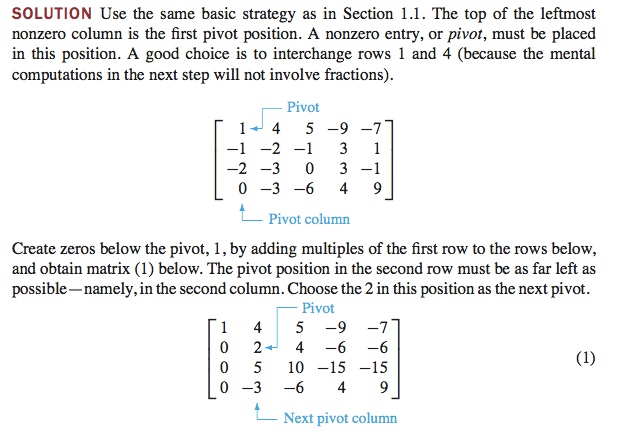
\includegraphics[scale=0.8]{figures_mvc/pivots_step_1}	
\end{center}

\begin{center}
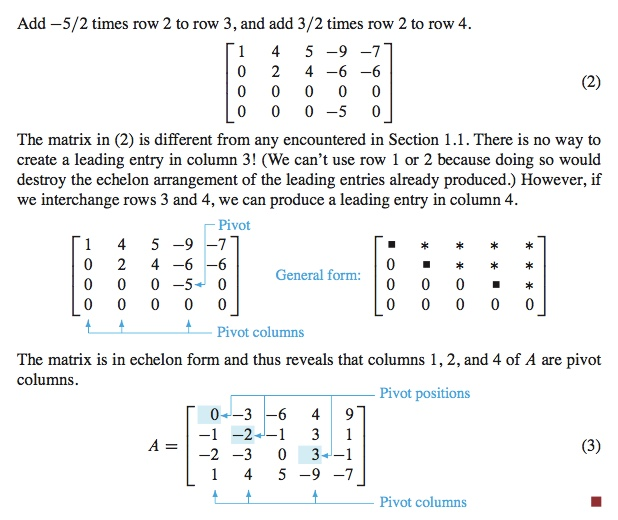
\includegraphics[scale=0.8]{figures_mvc/pivots_step_2}	
\end{center}
\end{example}

\subsection{Gauss-Jordan elimination}
In this section we introduce the \ti{Gauss-Jordan elimination} algorithm which will allow us to systematically reduce any matrix $A$ to its unique RREF, $U$. 

The algorithm consists of four steps, and it produces a matrix in REF. A fifth step produces a matrix in RREF. We illustrate the algorithm by an example.
 
\begin{align*}
	A=\begin{bmatrix}
		0 & 3 & -6 & 6 & 4 & -5 \\
		3 & -7 & 8 & -5 & 8 & 9 \\
		3 & -9 & 12 & -9 & 6 & 15
	\end{bmatrix}
\end{align*}

\begin{center}
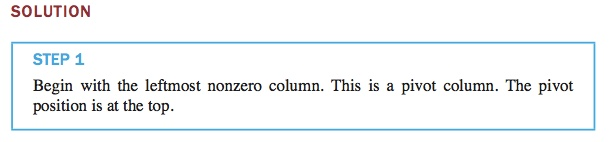
\includegraphics[scale=0.8]{figures_mvc/algo_step_1}	
\end{center}

\begin{center}
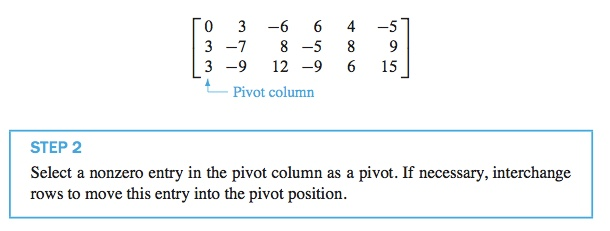
\includegraphics[scale=0.8]{figures_mvc/algo_step_2}	
\end{center}

\begin{center}
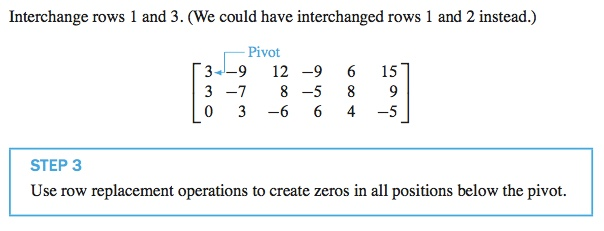
\includegraphics[scale=0.8]{figures_mvc/algo_step_3}	
\end{center}

\begin{center}
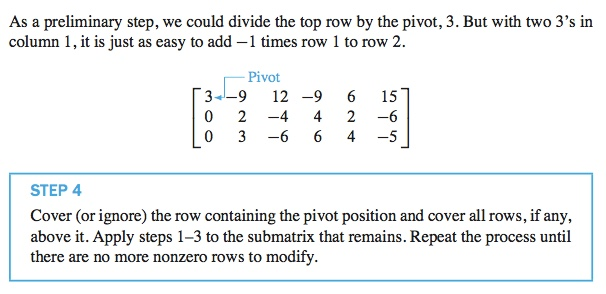
\includegraphics[scale=0.8]{figures_mvc/algo_step_4}	
\end{center}

\begin{center}
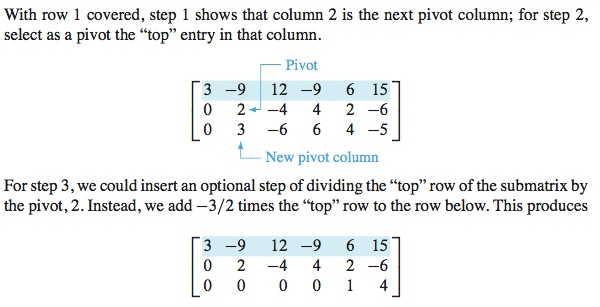
\includegraphics[scale=0.8]{figures_mvc/algo_step_5}	
\end{center}

\begin{center}
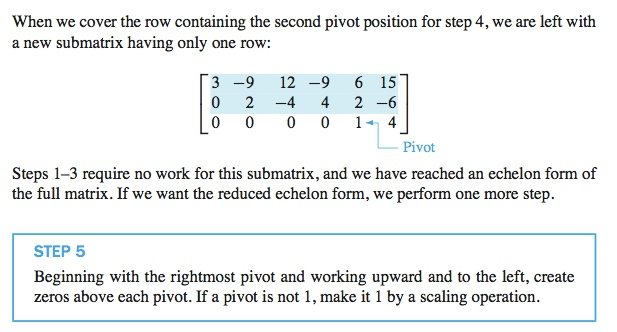
\includegraphics[scale=0.8]{figures_mvc/algo_step_6}	
\end{center}

\begin{center}
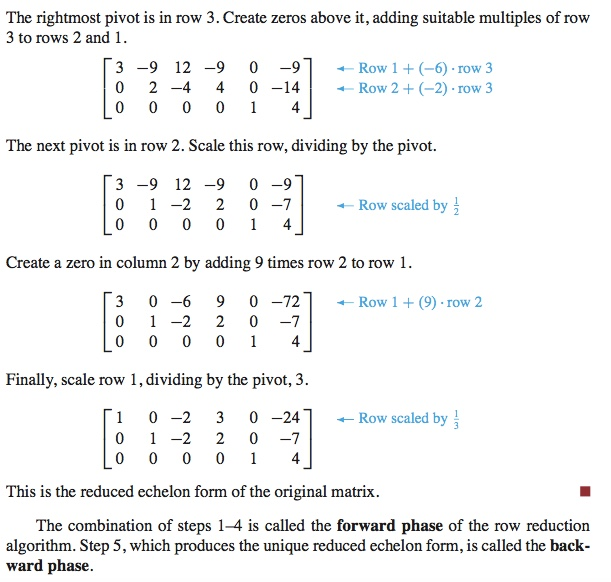
\includegraphics[scale=0.8]{figures_mvc/algo_step_7}	
\end{center}

\begin{exercise}
Row reduce the following matrices to RREF. Circle the pivot positions and pivot columns in the final matrix. \\
\vspace{0.25cm}
(a) $\begin{bmatrix}
	1 & 2 & 3 & 4 \\ 4 & 5 & 6 & 7 \\ 6 & 7 & 8 & 9
\end{bmatrix}$ \hspace{1.5cm} (b) $\begin{bmatrix}
	1 & 3 & 5 & 7 \\ 3 & 5 & 7 & 9 \\ 5 & 7 & 9 & 1
\end{bmatrix}$ \\
\vspace{0.25cm}
(c) $\begin{bmatrix}
	3 & -4 & 2 & 0 \\ -9 & 12 & -6 & 0 \\ -6 & 8 & -4 & 0
\end{bmatrix}$ \hspace{1.5cm} (d) $\begin{bmatrix}
	1 & -7 & 0 & 6 & 5 \\0 & 0 & 1 & -2 & -3 \\ -1 & 7 & -4 & 2 & 7
\end{bmatrix}$ 	
\end{exercise}

\subsection{Existence and uniqueness of solutions}
In this section we will answer the following two fundamental questions for any given linear system:
\begin{enumerate}
	\item Is the system consistent; that is, does at least one solution \ti{exist}.
	\item If a solution exists, is it the \ti{only} one; that is, is the solution \ti{unique}.
\end{enumerate}
\subsubsection{Homogeneous systems of linear equations}
A homogeneous system of linear equations $AX=0$ always has at least one solution, the \ti{trivial} solution, given by $x_1=x_2=\cdots=x_n=0$. Thus, \ti{a homogeneous system of linear equations is always consistent}. The fundamental question for a homogeneous system of linear equations is whether there exists a non-trivial solution.

Consider the system $RX=0$, where $R$ is an $m \times n$ matrix in reduced row echelon form. Let $1 \leq r \leq m$ and let $1,\cdots,r$ be the nonzero rows of $R$. The system $RX=0$ therefore consists of $r$ non-trivial equations. Letting $x_1,\cdots,x_r$ denote the first $r$ variables, and $u_i=x_{r+i}$, $i=1,\cdots,n-r$ denote the remaining $n-r$ free variables, the non-trivial equations take the form
\begin{align}
		x_1+\sum_{j=1}^{n-r}C_{1j}u_j&=0 \label{eq:non-triv_first} \\
		\vdots \hspace{1.8cm}& \hspace{0.5cm}\vdots \\
		x_r+\sum_{j=1}^{n-r}C_{rj}u_j&=0 \label{eq:non-triv_last}
	\end{align}
where each $x_i, i=1,\cdots,r$ occurs (with non-zero coefficient) only in the $i$th equation. All solutions to the system $RX=0$ are obtained by assigning any real numbers to $u_1,\cdots, u_{n-r}$ and then computing the values of $x_1,\cdots, x_r$ using \eqref{eq:non-triv_first} - \eqref{eq:non-triv_last}. This shows that \ti{if $r<n$, the system $RX=0$ has an infinite number of solutions}. If $r=n$, then $R$ is the $n \times n$ identity matrix and the system $RX=0$ has only the trivial solution. We thus have the following theorem:

\begin{thm}[Solution sets of homogeneous linear systems]\label{thm:solution_sets_of_homogeneous_linear_systems} \hspace{10cm}
	\begin{enumerate}[(a)]
		\item If $A$ is an $m \times n$ matrix and $m<n$, then the homogeneous system of linear equations $AX=0$ has a non-trivial solution (in fact, an infinite number of them). 
		\item If $A$ is an $n \times n$ (square) matrix, then $A$ is row-equivalent to the $n \times n$ identity matrix if and only if the system of equations $AX=0$ has only the trivial solution.
	\end{enumerate}
\end{thm}

\begin{pf}
	\begin{enumerate}[(a)]
		\item Let $R$ be the unique RREF of the matrix $A$. Since $A$ and $R$ are row-equivalent, the systems $AX=0$ and $RX=0$ have exactly the same solutions. As before, let $r$ be the number of non-zero rows in $R$. Then $r \leq m$, and since $m < n$, we have $r<n$. We will therefore have $n-r>0$ free variables, so $AX=0$ has a non-trivial solution. 
		\item $(\implies)$ If $A$ is row-equivalent to $I$, then $AX=0$ and $IX=0$ have the same solutions, hence $AX=0$ has only the trivial solution $X=0$. \\
		$(\impliedby)$ Suppose $AX=0$ has only the trivial solution. Let $R$ be the unique RREF of $R$, and let $r$ be the number of non-zero rows of $R$. Since $R$ is row-equivalent to $A$, $RX=0$ has only the trivial solution. Thus $r \geq n$. But since $R$ has $n$ rows, $r \leq n$, and therefore $r=n$. Since $R$ is in RREF, it is the $n \times n$ identity matrix.
	\end{enumerate}
\end{pf}
\begin{exercise}
Consider the system $RX=0$ with coefficient matrix
\begin{align*}
	R=\begin{bmatrix}
		1&0&0&2&7 \\
		0&1&0&-1&3 \\
		0&0&1&-4&5 \\
		0&0&0&0&0 
	\end{bmatrix}
\end{align*}
Verify the following:
\begin{enumerate}[(a)]
	\item The system $RX=0$ consists of $r$ non-trivial equations and $m-r$ trivial equations. Write out these equations.
	\item Show that the non-trivial equations take the form \eqref{eq:non-triv_first} - \eqref{eq:non-triv_last}. Indentify the basic variables $x_1,\cdots,x_r$, the free variables $u_1,\cdots,u_{n-r}$, and the coefficients $C_{ij}$ in these equations.
	\item Find the solution set and express it in parametric form.
\end{enumerate}	
\end{exercise}

\subsubsection{Inhomogeneous systems of linear equations}
So far we have used elementary row operations to solve homogeneous systems of linear equations. What, then, do elementary row operations do toward solving an inhomogeneous system of linear equations? Happily, it turns out that we solve an inhomogeneous system of linear equations in exactly the same way as a homogeneous one, with one minor modification.

\begin{defn}[Augmented matrix of an inhomogeneous linear system]\label{def:augmented_matrix}
The \ti{augmented matrix} of an inhomogeneous system of linear equations $AX=Y$ is the $m \times (n+1)$ matrix whose first $n$ columns are the columns of the coefficient matrix $A$ and whose last column is $Y$. We denote this matrix as $A'=[A|Y]$.
\end{defn}

\begin{example}\label{ex:augmented}
The augmented matrix of the inhomogeneous linear system
\begin{equation}\label{eq:inhom_system_example}
\begin{split}
	x_1-2x_2+x_3&=0 \\
	2x_2-8x_3&=8 \\
	5x_1-5x_3&=10 \\
\end{split}
\end{equation}
is given by
\begin{align*}
	A'=\left[\begin{array}{c c c | c}
		1&-2&1&0 \\
		0&2&-8&8 \\
		5&0&-5&10
	\end{array}\right]
\end{align*}	
\end{example}


Suppose we perform a sequence of elementary on the coefficient matrix $A$ of an inhomogeneous linear system $AX=Y$, arriving at it's unique reduced row echelon form, $R$. If we perform the same operations on $A'$, we will arrive at a matrix $R'$ in reduced row echelon form, whose first $n$ columns are those of $R$ and whose last column is the $m \times 1$ matrix $Z$ which results from applying the same sequence of elementary row operations to the matrix $Y$. By the same arguments as before, the system $RX=Z$ is equivalent to the original system $AX=Y$, and therefore we can read off the solution set from $RX=Z$.

\begin{exercise}
Verify that performing Gauss-Jordan elimination on the augmented matrix $A'$ of Example \ref{ex:augmented} gives
\begin{align*}
	\left[\begin{array}{c c c | c}
		1&-2&1&0 \\
		0&2&-8&8 \\
		5&0&-5&10
	\end{array}\right] \to \left[\begin{array}{c c c | c}
		1&0&0&1 \\
		0&1&0&0 \\
		0&0&1&-1
	\end{array}\right]
\end{align*}
	
This shows that the inhomogeneous system \eqref{eq:inhom_system_example} has the unique solution $(x_1,x_2,x_3)=(1,0,-1)$.
\end{exercise}


Therefore, \ti{to solve an inhomogeneous linear system $AX=Y$, we simply reduce the augmented matrix $A'=[A|Y]$ to its unique reduced row-echelon form, $R'=[R|Z]$, using Gauss-Jordan elimination (exactly as we do for the coefficient matrix $A$ for a homogeneous system). We then read off the solution set from the equivalent system $RX=Z$.}

While a homogeneous system of linear equations is always consistent, this need not be the case for an inhomogeneous system, even if the number of equations is fewer than the number of unknowns.

\begin{example}
Consider the inhomogeneous linear system
	\begin{align}
		x_1+3x_2+7x_3&=2 \label{eq:inhom_inconsistent_1} \\
		-2x_1-6x_2-14x_3&=-3 \label{eq:inhom_inconsistent_2}
	\end{align}
Replacing \eqref{eq:inhom_inconsistent_2} by $2\eqref{eq:inhom_inconsistent_1}+\eqref{eq:inhom_inconsistent_2}$ gives $0=1$, which is false for any $(x_1,x_2,x_3)$, so the system is inconsistent.
\end{example}

\begin{example}
Consider now the inhomogeneous linear system $AX=Y$ with augmented matrix
\begin{equation}\label{eq:inhom_general_example}
A'=\left[\begin{array}{c c c | c}
		1&-2&1&y_1 \\
			2&1&1&y_2 \\
			0&5&-1&y_3
	\end{array}\right]
\end{equation}
We would like to know:
\begin{enumerate}
	\item Under what condition does the solution exist?
	\item If a solution exists, is it unique?
\end{enumerate}
Performing elementary row operations on $A'$, we arrive at the row echelon matrix
\begin{equation}
	\left[\begin{array}{c c c | c}
		1&-2&1&y_1 \\
			0&5&-1&-2y_1+y_2 \\
			0&0&0&2y_1-y_2+y_3
	\end{array}\right].
\end{equation}
We see that the system is consistent only if $2y_1-y_2+y_3=0$. In this case, $x_3$ is a free variable, so the system has an infinite number of solutions.
\end{example}

This example is illustrative of the general case.

\begin{thm}[Existence and uniqueness for inhomogeneous systems]\label{thm:existence_and_uniqueness_for_inhomogeneous_systems} \hspace{10cm}
\begin{enumerate}[(a)]
	\item An inhomogeneous linear system is consistent if and only if the rightmost column of its augmented matrix is \ti{not} a pivot column - that is, if and only if any echelon form of the matrix has \ti{no} row of the form
	$$[0 \ \cdots \ 0\  b] \ \text{ with $b$ nonzero.}$$
	\item If an inhomogeneous linear system is consistent, then the solution set contains either $(i)$ a unique solution, when there are no free variables, or $(ii)$ infinitely many solutions, when there is at least one free variable.
\end{enumerate}
\fixme{Include a formal proof? Details are very similar to the homogeneous case, with the obvious modifications.}
\end{thm}


\subsection{Matrix operations}
In order to define operations on the set of matrices, it will help to take a slightly more formal view of a matrix. First, recall that a \ti{sequence} is just a function $f:\mathbb{N} \to \mathbb{R}$. Denoting $f(n)$ by $f_n$, we visualize a sequence as a list of real numbers $(f_1,f_2,f_3,\cdots)$, indexed by $n \in \mathbb{N}$.

\begin{example}
Let $f:\mathbb{N} \to \mathbb{R}$ be defined by $f(n)=\frac{1}{n}$. Then we write the sequence $(f_1,f_2,f_3)=(1,\frac{1}{2},\frac{1}{3},\cdots)$.	
\end{example}

\begin{defn}[Matrix]\label{def:matrix}
Let $\overline{n}=\{1,2,\cdots,n\}$. A \ti{matrix} is a function $A:\overline{m} \times \overline{n} \to \mathbb{R}$.	
\end{defn}

As we did with sequences, we denote $A(i,j)$ by $A_{ij}$. We then visualize the matrix $A$ as the rectangular array of the numbers $A_{ij}$ with $m$ rows and $n$ columns. Two matrices are \ti{equal} if they have the same size and if each of the corresponding entries are equal.

\begin{defn}[Diagonal matrix]
\fixme{Do we use this for anything here? Should this be moved?}
	The elements $A_{ii}$ (those with $i=j$) are the \ti{diagonal entries} of the matrix $A$. These form the \ti{main diagonal} of $A$. A matrix is said to be \ti{diagonal} if it is a square $(n \times n)$ matrix whose non-diagonal entries ($A_{ij}$ with $i \neq j$) are all zero.	
\end{defn}

\begin{example}
The $n \times n$ \ti{identity matrix} is the diagonal matrix $I$ with elements
\begin{align*}
	I_{ij}=\delta_{ij}=\begin{cases}
		1, \text{ if } i=j, \\
		0, \text{ if } i \neq j
	\end{cases}	
	\end{align*}
where $\delta$ is called the \ti{Kronecker delta symbol}.
\end{example}

\subsubsection{Matrix addition and scalar multiplication}
The definition of a matrix in \ref{def:matrix} makes it clear how to define addition and scalar multiplication of matrices; namely, we define these operations pointwise, the same way we always do for any function: 
\begin{align*}
	(f+g)(a) &=f(a)+g(a) \\
	(cf)(a) &=cf(a) 
\end{align*}

\begin{defn}[Matrix addition]
	If $A$ and $B$ are two $m \times n$ matrices, then the matrix $A+B$ has elements $(A+B)_{ij}=A_{ij}+B_{ij}$.
\end{defn}
Note that matrix addition is only defined if $A$ and $B$ are two matrices of the same size.
\begin{exercise}
	Let $A=\begin{bmatrix}
	4&0&5 \\ -1&3&2
\end{bmatrix}, B=\begin{bmatrix}
	1&1&1\\3&5&7
\end{bmatrix}$, and $C=\begin{bmatrix}
	2&-3 \\ 0&1
\end{bmatrix}$. Determine whether $A+B$ and $A+C$ are defined. If so, compute them.
\end{exercise}


\begin{defn}[Scalar multiplication of a matrix]
	If $A$ is an $m \times n$ matrix and $c$ is any scalar, then the matrix $cA$ has elements $(cA)_{ij}=cA_{ij}$.
\end{defn}

\begin{exercise}
Let $A$ and $B$ be the same as in the previous exercise. Compute $2B$ and $A-2B$.	
\end{exercise}

The usual rules of algebra apply to sums and scalar multiples of matrices, as the next theorem shows.

\begin{thm}[Properties of matrix addition and scalar multiplication]
Let $A,B,$ and $C$ be matrices of the same size, and let $r$ and $s$ be scalars.
	\begin{enumerate}[(i)]
		\item $A+B=B+A$ (matrix addition is commutative)
		\item $(A+B)+C=A+(B+C)$ (matrix addition is associative)
		\item $A+0=A$ (the zero matrix is an additive identity)
		\item $r(A+B)=rA+rB$ (scalar multiplication distributes over matrix addition)
		\item $(r+s)A=rA+sA$ (scalar multiplication distributes over scalar addition)
		\item $r(sA)=(rs)A$ (associativity of scalar multiplication)
	\end{enumerate}
\end{thm}


\begin{pf}
For each of these we need to show that $(1)$ the matrix on the left and right hand side of each equation has the same size, and $(2)$ each of the corresponding entries are equal. Condition $(1)$ holds for each since $A,B,$ and $C$ are all the same size. Condition $(2)$ holds in each case because of the corresponding properties of real numbers. For example, property $(i)$ holds for matrices $A$ and $B$ since $A_{ij}+B_{ij}=B_{ij}+A_{ij}$ holds for real numbers $A_{ij}$ and $B_{ij}$. The remaining properties are checked similarly and are left as an exercise.
\end{pf}

\subsubsection{Matrix multiplication}
We have seen in the previous sections that the process of forming linear combinations of the rows of a matrix is a fundamental one. We now introduce a systematic way of doing this. 

Let $B$ be an $n \times p$ matrix with rows $\beta_1,\beta_2,\cdots, \beta_n$. Denote the $j$th entry of the $i$th row by $B_{ij}$. For example, if
\begin{align*}
	B=\begin{bmatrix}
		5&-1&2 \\ 15&4&8
	\end{bmatrix}
\end{align*}
then $n=2, p=3, \beta_1=(5,-1,2), B_{12}=-1$, etc. Now construct an $m \times n$ matrix $C$ with rows $\gamma_1, \gamma_2,\cdots, \gamma_m$ by forming certain linear combinations of the rows of $B$. For example, let $C$ be given by
\begin{align*}
	C=\begin{bmatrix}
		2(5,-1,2)-1(15,4,8)\\
		1(5,-1,2)+3(15,4,8)\\
		-2(5,1,2)+6(15,4,8)
	\end{bmatrix}=\begin{bmatrix}
		-5&-6&-4 \\
		50&11&26 \\
		80&22&44
	\end{bmatrix}
\end{align*} 
Denoting the $i$th multiple of $j$th row of $B$ by $A_{ij}$, the $i$th row of $C$ is given by $\gamma_i=A_{i1}\beta_1+A_{i2}\beta_2+\cdots+A_{in}\beta_n=\sum_{j=1}^nA_{ij}\beta_j$. We see that the rows of $C$ are determined by $mn$ scalars $A_{ij}$ which are themselves the entries of an $m \times n$ matrix 
	\begin{align*}
		A=\begin{bmatrix}
			2&-1\\1&3\\-2&6
		\end{bmatrix}
	\end{align*}
Letting $C_{ik}$ denote the $k$th entry of the $i$th row of $C$, we see that $C_{ik}=\sum_{j=1}^n A_{ij}B_{jk}$. We define this matrix $C$ to be the \ti{product} of matrices $A$ and $B$.

\begin{defn}[Matrix multiplication]\label{def:matrix_multiplication}
	Let $A$ be an $m \times n$ matrix and $B$ be an $n \times p$ matrix. The \ti{product} of $A$ and $B$ is the $m \times p$ matrix $C$ whose $(i,j)$-entry is $C_{ij}=\sum_{k=1}^n A_{ik}B_{kj}$.
\end{defn}

\begin{example}[Row-column rule for matrix multiplication]
	One can remember this definition by the following ``row-column" rule for computing $AB$: the entry in row $i$ and column $j$ of $AB$ is the sum of the products of corresponding entries from row $i$ of $A$ and column $j$ of $B$. That is, the $(i,j)$-entry of $AB$ is given by
\begin{equation}
	(AB)_{ij}=A_{i1}B_{1j}+A_{i2}B_{2j}+\cdots+A_{in}B_{nj}	
\end{equation}

\end{example}



\begin{example}
Taking $A$ and $B$ to be the matrices in the discussion at the beginning of this section, their product is  
\begin{align*}
	C&=AB \\
	&=\begin{bmatrix}
			2&-1\\1&3\\-2&6
		\end{bmatrix}\begin{bmatrix}
		5&-1&2 \\ 15&4&8
	\end{bmatrix} \\
	&=\begin{bmatrix}
		-5&-6&-4 \\
		50&11&26 \\
		80&22&44
	\end{bmatrix}
\end{align*}
\end{example}

Notice that the product of two matrices is only defined if the number of \ti{columns} in the first matrix coincides with the number of \ti{rows} in the second matrix. In this case, multiplying an $n \times p$ matrix and a $p \times m$ matrix gives an $n \times m$ matrix.

\begin{exercise}
	If $A$ is a $3 \times 5$ matrix and $B$ is a $5 \times 2$ matrix, what are the sizes of $AB$ and $BA$, if they are defined?	
\end{exercise}

\begin{exercise}
Let $A=\begin{bmatrix}
	2&3\\1&-5
\end{bmatrix}$ and $B=\begin{bmatrix}
	4&3&6 \\1&-2&3
\end{bmatrix}$. Compute $AB$.	
\end{exercise}

Note that this definition of matrix multiplication agrees with our notation $AX=Y$ for a linear system of equations: $A$ is an $m \times n$ matrix, $X$ is an $ n \times 1$ matrix, and $Y$, which is the product of $A$ and $X$ is an $m \times 1$ matrix. 
	\begin{align*}
		\begin{bmatrix}
			A_{11} & A_{12} & \cdots & A_{1n} \\
			\vdots & &  & \vdots \\
			A_{m1} & A_{m2} & \cdots & A_{mn}
		\end{bmatrix}\begin{bmatrix}
			x_1 \\ x_2 \\ \vdots \\ x_n
		\end{bmatrix}=\begin{bmatrix}
			y_1 \\ y_2 \\ \vdots \\ y_m
		\end{bmatrix}
	\end{align*}

\begin{defn}[Power of a matrx]
	If $A$ is an $n\times n$ matrix and $k$ is a positive integer, then the \ti{$k$th power of $A$}, $A^k$, is the product of $k$ copies of $A$:
\begin{align*}
	A^k=\underbrace{A \cdots A}_{\text{$k$ times}}.
\end{align*}
\end{defn}

\begin{thm}[Properties of matrix multiplication]\label{thm:properties_of_matrix_multiplication}
	Let $A$ be an $m \times n$ matrix, and let $B$ and $C$ have sizes for which the indicated sums and products are defined. Then the following hold for all such matrices $A,B,$ and $C$.
\begin{enumerate}[(i)]
	\item $(AB)C=A(BC)$ (associative law of multiplication)
	\item $A(B+C)=AB+AC$ (left distributive law)
	\item $(B+C)A=BA+CA$ (right distributive law)
	\item $r(AB)=(rA)B=A(rB)$ for any scalar $r$
	\item $I_mA=A=AI_n$ (identity for matrix multiplication)
\end{enumerate}
\end{thm}

\begin{pf}
As before, for each of these we need to check that (1) both sides are matrices of the same size, and (2) the corresponding matrix elements on each side are all equal. 

(i) For $AB$ to be defined, $B$ must be an $n \times p$ matrix, for some $p$. Then, for $BC$ to be defined, $C$ must be $p \times q$ matrix. We therefore have 
\begin{align*}
	AB: (m \times n)(n \times p)&=m \times p \\
	BC: (n \times p)(p \times q)&=n \times q
\end{align*}
so
\begin{align*}
	(AB)C: (m \times p)(p \times q)&=m \times q \\
	A(BC): (m \times n)(n \times q)&=m \times q
\end{align*}
hence both sides have the same size. \\
\\

Applying the definition of matrix multiplication, we have
\begin{align*}
	[(AB)C]_{ij}&=\sum_{\ell=1}^p(AB)_{i\ell}C_{\ell j} \\
	&=\sum_{\ell=1}^p\sum_{k=1}^n (A_{ik}B_{k\ell})C_{\ell j} \\
	&=\sum_{\ell=1}^p\sum_{k=1}^n A_{ik}(B_{k\ell}C_{\ell j}) \text{ (by associativity in $\mathbb{R}$)}\\
	&=\sum_{k=1}^nA_{ik}(BC)_{kj} \\
	&=[A(BC)]_{ij},
\end{align*}
so the corresponding entries are equal, showing that (i) holds. Properties (ii) - (v) are checked similarly, and are left as exercises.	
\end{pf}

We have seen in theorem Theorem \ref{thm:properties_of_matrix_multiplication} that some of the properties of multiplication of real numbers also hold for matrices. However, it is not true that \ti{all} such properties hold for matrix multiplication, as the next three examples show.

\begin{example}[Matrix multiplication is not commutative] 
	Let $A=\begin{bmatrix}
		5&1\\3&-2
	\end{bmatrix}$ and $B=\begin{bmatrix}
		2&0 \\ 4&3
	\end{bmatrix}$. Then $AB=\begin{bmatrix}
	16 & 9 \\ -18 & -15
\end{bmatrix}$ and  $BA=\begin{bmatrix}
	4 & 6 \\ 11 & -3
\end{bmatrix}$. Since $AB \neq BA$, this example shows that matrix multiplication is not, in general, commutative.
\end{example}

\begin{example}[Matrix multiplication does not satisfy cancellation laws]
For real numbers, the cancellation law says that if $AB=AC$, then $B=C$. This does not hold, in general, for matrices. As an example, let $A=\begin{bmatrix}
		2&-3\\-4&6
	\end{bmatrix},$ $B=\begin{bmatrix}
		8&4\\5&5
	\end{bmatrix},$ and $C=\begin{bmatrix}
		5&-2\\3&1
	\end{bmatrix}$.	We see that $AB=BC=\begin{bmatrix}
	1 & -7 \\ -2 & 14
\end{bmatrix}$, but $B \neq C$. One can show similarly that the other cancellation law ($BA=CA \implies B=C$) also does not hold in general for matrices.
\end{example}

\begin{example}[Zero products do not imply one matrix is zero]
	For real numbers, if $AB=0$ then either $A=0$ or $B=0$. To see that this does not hold, in general, for matrices, let $A=\begin{bmatrix}
		3&-6 \\ -1&2
	\end{bmatrix}$ and $B=\begin{bmatrix}
	2 & 2 \\ 1 & 1
\end{bmatrix}$. Then $AB=0$, but neither $A$ nor $B$ is the zero matrix. 
\end{example}

\subsubsection{Transpose of a matrix}

\begin{defn}[Transpose of a matrix]
	Given an $m \times n$ matrix $A$, the \ti{transpose} of $A$ is the $n \times m$ matrix, denoted $A^T$, whose columns are formed from the corresponding rows of $A$, that is, given $A$, $A^T$ is the matrix with elements $(A^T)_{ij}=A_{ji}$. 
\end{defn}

\begin{example}
	If $A=\begin{bmatrix}
	-5&2\\1&-3 \\ 0&4
\end{bmatrix}$, then $A^T=\begin{bmatrix}
	-5&1&0 \\ 2&-3&4
\end{bmatrix}$.
\end{example}

\begin{thm}[Properties of $A^T$]
	Let $A$ and $B$ be matrices whose sizes are appropriate for the following sums and products to be defined. Then
\begin{enumerate}[(i)]
	\item $(A^T)^T=A$
	\item $(A+B)^T=A^T+B^T$
	\item For any scalar $r$, $(rA)^T=rA^T$
	\item $(AB)^T=B^TA^T$
\end{enumerate}
\end{thm}

\begin{pf}
Clearly the matrices on each side are the same size since $A$ and $B$ are the same size. All that is left is to check that the corresponding matrix elements are equal in each case. We will do this for (iv). The proofs for (i)-(iii) are checked similarly, and are left as exercises. 
\begin{align*}
	[(AB)^T]_{ij}&=(AB)_{ji} \\
	&=\sum_{k=1}^n A_{jk}B_{ki} \\
	&=\sum_{k=1}^n B_{ki}A_{jk} \ (\text{by commutativity in } \mathbb{R}) \\
	&=\sum_{k=1}^n B^T_{ik}A^T_{kj} \\
	&=[B^TA^T]_{ij}	
\end{align*}
This proves property (iv).
\end{pf}

\subsubsection{Trace of a matrix}
\fixme{Is this a good place for this?}


\subsection{Invertible matrices}
\subsubsection{Elementary matrices}
If $B$ is a given matrix and $C$ is obtained from $B$ by  an elementary row operation, then each row of $C$ is a linear combination of the rows of $B$, and hence there is a matrix $A$ such that $AB=C$. In general there are many such matrices $A$, and among all of these it is convenient and possible to choose one having a number of special properties. First, we need to introduce a class of matrices. \fixme{Give a better introduction here.} 

\begin{defn}[Elementary matrix]\label{def:elementary_matrix}
	An $n \times n$ (square) matrix is said to be an \ti{elementary matrix} if it can be obtained from the $n \times n$ identity matrix by means of a single elementary row operation.
\end{defn}

\begin{exercise}
Verify that the complete list of $2 \times 2$ elementary matrices is 
	\begin{align*}
	\begin{bmatrix}
		0 & 1 \\ 1 & 0
	\end{bmatrix}, \begin{bmatrix}
		1 & c \\ 0 & 1
	\end{bmatrix}, \begin{bmatrix}
		1 & 0 \\ c & 1
	\end{bmatrix}, 
	 \begin{bmatrix}
		c & 0 \\ 0 & 1
	\end{bmatrix} (c \neq 0), \begin{bmatrix}
		1 & 0 \\ 0 & c
	\end{bmatrix} (c \neq 0)
\end{align*}
\end{exercise}

\begin{thm}[Elementary row operations are represented by elementary matrices]
If $e$ is an elementary row operation and $E$ the $n \times n$ elementary matrix $E=e(I)$, then for every $m \times n$ matrix $A$, $e(A)=EA$.	
\end{thm}

\begin{pf}
We consider each type of elementary row operation separately.

(i) Suppose $r \neq s$ and let $e$ be the elementary row operation which replaces row $r$ by row $r$ plus $c$ times row $s$. We need to show that $EA=e(A)$. We can write the elements of the corresponding elementary matrix $E$ as 
	 \begin{align*}
	 	E_{ik}=\begin{cases}
	 		\delta_{ik}, &i \neq r \\
	 		\delta_{rk}+c\delta_{sk}, &i=r.
	 	\end{cases}
	 \end{align*}
Then, if $i \neq r$, 
\begin{align*}
	(EA)_{ij}=\sum_{k=1}^m E_{ik}A_{kj} = \sum_{k=1}^m\delta_{ik}A_{kj}=A_{ij}
\end{align*}
and for $i=r$,
\begin{align*}
	(EA)_{rj}=\sum_{k=1}^m E_{rk}A_{kj} =\sum_{k=1}^m(\delta_{rk}+c\delta_{sk})A_{kj} =A_{rj}+cA_{sj}
\end{align*}
which shows $EA=e(A)$, as desired.

(ii) Suppose $r \neq s$ and let $e$ be the elementary row operation which exchanges rows $r$ and $s$. The elements of the corresponding elementary matrix are given by
	 \begin{align*}
	 	E_{ik}=\begin{cases}
	 		\delta_{ik}, &i \neq r,s \\
	 		\delta_{rk}, &i=s \\
	 		\delta_{sk}, &i=r.
	 	\end{cases}
	 \end{align*}
Then, if $i \neq r,s$, 
\begin{align*}
	(EA)_{ij}=\sum_{k=1}^m E_{ik}A_{kj} = \sum_{k=1}^m\delta_{ik}A_{kj}=A_{ij}
\end{align*}
if $i=r$,
\begin{align*}
	(EA)_{rj}=\sum_{k=1}^m E_{rk}A_{kj} =\sum_{k=1}^m\delta_{sk}A_{kj} =A_{sj}
\end{align*}
and if $i=s$,
\begin{align*}
	(EA)_{sj}=\sum_{k=1}^m E_{sk}A_{kj} =\sum_{k=1}^m\delta_{rk}A_{kj} =A_{rj}
\end{align*}
which shows $EA=e(A)$.

(iii) Let $e$ be the elementary row operation which multiplies rows $r$ by $c$, $c\neq 0$. We need to show that $EA=e(A)$. The corresponding elementary matrix can be written as 
	 \begin{align*}
	 	E_{ik}=\begin{cases}
	 		\delta_{ik}, &i \neq r \\
	 		c\delta_{rk}, &i=r. 
	 	\end{cases}
	 \end{align*}
Then, if $i \neq r$, 
\begin{align*}
	(EA)_{ij}=\sum_{k=1}^m E_{ik}A_{kj} = \sum_{k=1}^m\delta_{ik}A_{kj}=A_{ij}
\end{align*}
if $i=r$,
\begin{align*}
	(EA)_{rj}=\sum_{k=1}^m E_{rk}A_{kj} =\sum_{k=1}^m(c\delta_{rk})A_{kj} =cA_{rj}
\end{align*}
which shows $EA=e(A)$.	
\end{pf}

\begin{exercise}
Let $E_1=\begin{bmatrix}
	1&0&0 \\ 0&1&0 \\ -4&0&1
\end{bmatrix}, E_2=\begin{bmatrix}
	0&1&0 \\ 1&0&0 \\ 0&0&1
\end{bmatrix}$, and $E_3=\begin{bmatrix}
	1&0&0 \\ 0&1&0 \\ 0&0&5
\end{bmatrix}$, and let $A$ be an arbitrary $3 \times 3$ matrix. Compute 
$E_1A, E_2A,$ and $E_3A$, and describe how these products can be obtained by elementary row operations on $A$.	
\end{exercise}

\begin{cor}
Let $A$ and $B$ be $m \times n$ matrices. Then $B$ is row-equivalent to $A$ if and only if $B=PA$, where $P$ is a product of $m \times m$ elementary matrices.	
\end{cor}

\begin{pf}
$(\implies)$ Suppose $B$ is row-equivalent to $A$. Let $E_1, E_2, \cdots, E_s$ be the elementary matrices corresponding to some sequence of elementary row operations which carries $A$ into $B$. Then $B=(E_s \cdots E_2 E_1)A$.

$(\impliedby)$ Suppose $B=PA$ where $P=E_s \cdots E_2E_1$ and the $E_i$ are $m \times m$ elementary matrices. Then $E_1 A$ is row-equivalent to $A$, and $E_2(E_1 A)$ is row-equivalent to $E_1 A$, so by transitivity $E_2E_1A$ is row-equivalent to $A$. It follows by induction that $(E_s \cdots E_1)A$ is row-equivalent to $A$.	
\end{pf}

\fixme{Exercise here?}

\subsubsection{Invertible matrices}
Suppose $P$ is an $m \times m$ matrix which is a product of elementary matrices. Then, for each $m \times n$ matrix $A$, the matrix $B=PA$ is row-equivalent to $A$. By symmetry, $A$ is therefore row-equivalent to $B$ and there is a product $Q$ of elementary matrices such that $A=QB$. In particular, this is true when $A$ is the $m \times m$ identity matrix. 

In other words, there is an $m \times m$ matrix $Q$, which is itself a product of elementary matrices, such that $QP=I$. As we shall soon see, the existence of a $Q$ with $QP=I$ is equivalent to the fact that $P$ is a product of elementary matrices.

\begin{defn}[Invertible matrix]
	Let $A$ be an $n \times n$ matrix. An $n \times n$ matrix $B$ such that $BA=I$ is called a \ti{left inverse} of $A$; an $n \times n$ matrix $B$ such that $AB=I$ is called a \ti{right inverse} of $A$. If $AB=BA=I$, then $B$ is called a \ti{two-sided inverse} (or just \ti{inverse}) of $A$ and $A$ is said to be \ti{invertible}.
\end{defn}

\begin{exercise}
Let $A=\begin{bmatrix}
	2&5 \\ 3&8
\end{bmatrix}$ and $B=\begin{bmatrix}
	8&-5 \\ -3&2
\end{bmatrix}$. Show that $B$ is a two-sided inverse for $A$.	
\end{exercise}

\begin{thm}[Uniqueness of inverses]\label{thm:uniqueness_of_inverses}
	If $A$ has a left inverse $B$ and a right inverse $C$, then $B=C$. 
\end{thm}

\begin{pf}
Suppose $BA=I$ and $AC=I$. Then
\begin{align*}
	B=BI=B(AC)=(BA)C=IC=C. 
\end{align*}	
\end{pf}

Thus, if $A$ has a two-sided inverse, then it is unique. We denote the unique two-sided inverse by $A^{-1}$ and call it \ti{the inverse} of $A$.

\begin{thm}[Properties of $A^{-1}$]\label{thm:properties_of_A_inverse} \hspace{10cm}
		\begin{enumerate}[(i)]
		\item If $A$ is invertible, so is $A^{-1}$ and $(A^{-1})^{-1}=A$.
		\item If both $A$ and $B$ are invertible, so is $AB$, and $(AB)^{-1}=B^{-1}A^{-1}$.
		\item If $A$ is invertible, so is $A^T$ and $(A^T)^{-1}=(A^{-1})^T$.
	\end{enumerate}
\end{thm}

\begin{pf} 
(i) Follows immediately from the symmetry of the definition. 

(ii) $(B^{-1}A^{-1})(AB)=B^{-1}(A^{-1}A)B=B^{-1}B=I$. By uniqueness of inverses, $(AB)^{-1}=B^{-1}A^{-1}$.

(iii) $(A^{-1})^TA^T=(AA^{-1})^T=I^T=I$. By uniqueness of inverses, $(A^{-1})^T=(A^T)^{-1}$. 

Generalizing (ii), any finite product of invertible matrices is invertible, with inverse
\begin{align*}
	(A_1A_2\cdots A_s)=A_s^{-1} \cdots A_2^{-1}A_1^{-1}
\end{align*}	
\end{pf}

\begin{thm}[Elementary matrices are invertible]\label{thm:elementary_matrices_are_invertible}
An elementary matrix $E$ is invertible. The inverse of $E$ is the elementary matrix of the same type that transforms $E$ back into $I$.
\end{thm}

\begin{pf}
Let $E$ be the elementary matrix corresponding to the elementary row operation $e$. If $e'$ is the inverse operation of $e$ and $E'=e'(I)$, then $EE'=e(E')=e(e'(I))=I$, so $E$ is invertible and $E'=E^{-1}$.	
\end{pf}

\begin{example}
\begin{enumerate}[(a)]
	\item $\begin{bmatrix}
		0&1 \\ 1&0
	\end{bmatrix}^{-1}=  \begin{bmatrix}
		0 & 1 \\ 1 & 0
	\end{bmatrix}$
	\item $\begin{bmatrix}
		1&c \\ 0&1
	\end{bmatrix}^{-1}= \begin{bmatrix}1 & -c \\ 0 & 1 \end{bmatrix}$
	\item $\begin{bmatrix}
		1&0 \\ c&1
	\end{bmatrix}^{-1}=\begin{bmatrix}
		1 & 0 \\ -c & 1
	\end{bmatrix}$
	\item When $c \neq 0$,
	$\begin{bmatrix}
		c&0 \\ 0&1
	\end{bmatrix}^{-1}=\begin{bmatrix}
		c^{-1} & 0 \\ 0 & 1
	\end{bmatrix},$ \hspace{0.5cm} $\begin{bmatrix}
		1&0 \\ 0 &c
	\end{bmatrix}^{-1}= \begin{bmatrix}
		1 & 0 \\ 0 & c^{-1}
	\end{bmatrix}.$
\end{enumerate}
\end{example}

\begin{thm}[Invertible matrix theorem]\label{thm:invertible_matrix_theorem}
	If $A$ is an $n \times n$ matrix, the following are equivalent.
	\begin{enumerate}[(i)]
		\item $A$ is invertible.
		\item $A$ is row-equivalent to the $n \times n$ identity matrix.
		\item $A$ is a product of elementary matrices.
	\end{enumerate} 	
\end{thm}

\begin{pf}
We will show that $(i) \implies (ii) \implies (iii) \implies (i)$. Assume $(i)$ is true. Let $R$ be the RREF of $A$. Then $R=E_k\cdots E_2 E_1 A$, where $E_1,\cdots,E_k$ are elementary matrices. Since each $E_j$ is invertible, we have $A=E_1^{-1} \cdots E_k^{-1}R$. Since products of invertible matrices are invertible, we see that $A$ is invertible if and only if $R$ is invertible. Since $R$ is a square matrix in RREF, $R$ is invertible iff it is the $n \times n$ identity matrix. Hence, $(i) \implies (ii)$. $(iii)$ follows immediately from $(ii)$. $(i)$ follows immediately from $(iii)$.	
\end{pf}

\begin{cor}[How to compute $A^{-1}$]\label{cor:how_to_compute_a_inverse}
If $A$ is an invertible $n \times n$ matrix and if a sequence of elementary row operations reduces $A$ to the identity, then that same sequence of operations when applied to $I$ yields $A^{-1}$.	
\end{cor}

\begin{pf}
If $E_k \cdots E_1 A=I$, where each $E_j$ is an elementary matrix, then multiplying both sides on the right by $A^{-1}$ gives $E_k \cdots E_1 I=A^{-1}$.	
\end{pf}

Corollary \ref{cor:how_to_compute_a_inverse} gives an algorithm to compute $A^{-1}$: we simply row reduce the augmented matrix $[A|I]$. If $A$ is row-equivalent to $I$, then $[A|I]$ is row-equivalent tp $[I|A^{-1}]$. Otherwise, $A$ does not have an inverse.

\begin{example}
We find the inverse of the matrix $A=\begin{bmatrix}
	0&1&2 \\ 1&0&3 \\ 4&-3&8
\end{bmatrix}$ by performing Gauss-Jordan elimination on the augmented matrix
\begin{align*}
\left[	\begin{array}{c c c | c c c}
		0 & 1 & 2 & 1 & 0 & 0 \\
		1 & 0 &3 & 0 & 1 & 0 \\
		4 & -3 & 8 & 0 & 0 & 1
	\end{array}\right],
\end{align*} which gives \begin{align*}
\left[	\begin{array}{c c c | c c c}
		1 & 0 & 0 & -\frac{9}{2} & 7 & -\frac{3}{2} \\
		0 & 1 & 0 & -2 & 4 & -1 \\
		0 & 0 & 1 & \frac{3}{2} & -2 & \frac{1}{2} 
	\end{array}\right]
\end{align*}
so $A^{-1}=\begin{bmatrix}
	-\frac{9}{2} & 7 & -\frac{3}{2} \\
	-2 & 4 & -1 \\
	\frac{3}{2} & -2 & \frac{1}{2}
\end{bmatrix}$.	
\end{example}

\begin{exercise}
Find the inverse of the matrix $A=\begin{bmatrix}
	3 & 1 & -2 \\ 1 & 0 & 2 \\ -1 & -2 & 4
\end{bmatrix}$, if it exists.	
\end{exercise}

Let us now make some general statements about the invertibility of square matrices. The simplest square matrix is a $1 \times 1$ matrix, which is just a number, $a_{11}$. Obviously, a $1 \times 1$ matrix is invertible if and only if $a_{11} \neq 0$.

Let us now consider a general $2 \times 2$ matrix $A$:
\begin{align*}
	A=\begin{bmatrix}
		a_{11} & a_{12} \\ a_{21} & a_{22}
	\end{bmatrix}.
\end{align*}
and see what happens when its augmented matrix $A$ is row-reduced. For $A$ to be invertible each column must have a pivot, so we cannot have $a_{11}$ and $a_{12}$ both zero. We therefore assume $a_{11} \neq 0$ (swapping $R1$ and $R2$, if necessary). If we multiply the second row by $a_{11}$ and then subtract $a_{21} \times R1$ from $R2$, we find that $A$ is row-equivalent to the following two matrices:
\begin{align*}
	\begin{bmatrix}
		a_{11}& a_{12} \\ a_{11}a_{12} & a_{11}a_{22}
	\end{bmatrix} \sim \begin{bmatrix}
		a_{11}& a_{12} \\ 
		0 & a_{11}a_{22}-a_{12}a_{21}
	\end{bmatrix}
\end{align*} 
To have a pivot in the $(2,2)$-position, we must have that
\begin{equation}
	a_{11}a_{22}-a_{12}a_{21} \neq 0.
\end{equation}

\begin{defn}[Determinant of a $2 \times 2$ matrix]
Let $A$ be a $2 \times 2$ matrix. The quantity $a_{11}a_{22}-a_{12}a_{21}$ is called the \ti{determinant} of $A$, and is denoted $\det A$.
\end{defn}

\begin{prop}[Invertibility of a $2 \times 2$ matrix]\label{prop:2_by_2_invertibility}
A $2 \times 2$ matrix $A$ is invertible if and only if $\det A \neq 0$.
\end{prop}

\begin{pf}
We have just seen that if $A$ is invertible, then $\det A \neq 0$. 

To prove the converse, assume $\det A \neq 0$. Since $\det A=a_{11}a_{22}-a_{12}a_{21}$, either $a_{11} \neq 0$ or $a_{12} \neq 0$. Assuming $a_{11} \neq 0$, we can divide by $a_{11}$ to solve for $a_{22}$:
\begin{align*}
	a_{22}=\frac{\det A+a_{12}a_{21}}{a_{11}}
\end{align*} 
	and therefore
	\begin{align*}
		A=\begin{bmatrix}
			a_{11} & a_{12} \\
			a_{21} & \frac{\det A+a_{12}a_{21}}{a_{11}}
		\end{bmatrix}.
	\end{align*}
Multiplying $R2$ by $a_{11}$ and subtracting $a_{21} \times R1$ from the new $R2$, we find
\begin{align*}
	A \sim \begin{bmatrix}
		a_{11} & a_{12} \\
		a_{11}a_{21} & \det A + a_{12}a_{21}
	\end{bmatrix} \sim \begin{bmatrix}
		a_{11} & a_{12} \\
		0 & \det A
	\end{bmatrix}
\end{align*}
Hence, $A$ has two pivot columns, and is therefore invertible.
\end{pf}

The previous proposition turns out to hold for all square matrices. That is, the invertibility of any square matrix is determined by a single combination of its entries, and the matrix is invertible as long as this combination is not zero. Thus, if we know how to compute the determinant of a square matrix, we can check immediately if the matrix is invertible by checking whether the determinant is different from zero. 

Let us see this for the $3 \times 3$ case. A general $3 \times 3$ matrix can be written as 
\begin{align*}
	A=\begin{bmatrix}
		a_{11} & a_{12} & a_{13} \\
		a_{21} & a_{22} & a_{23} \\
		a_{31} & a_{32} & a_{33}
	\end{bmatrix}
\end{align*}
As before, the first column must be a pivot column if $A$ is invertible, so let us again assume that $a_{11} \neq 0$ (again, we can achieve this by swapping rows, if necessary). If we multiply the second and third rows of $A$ by $a_{11}$ and then subtract appropriate multiples of the first row from the other two rows, we find that $A$ is row-equivalent to the following two matrices:
\begin{align*}
	\begin{bmatrix}
		a_{11} & a_{12} & a_{13} \\
		a_{11}a_{21} & a_{11}a_{22} & a_{11}a_{23} \\
		a_{11}a_{31} & a_{11}a_{32} & a_{11}a_{33} 
	\end{bmatrix} \sim \begin{bmatrix}
		a_{11} & a_{12} & a_{13} \\
		0 & a_{11}a_{22}-a_{12}a_{21} & a_{11}a_{23}-a_{13}a_{21} \\
		0 & a_{11}a_{32}-a_{12}a_{31} & a_{11}a_{33}-a_{13}a_{31}
	\end{bmatrix}
\end{align*}
For $A$ to be invertible, either the $(2,2)$- or $(3,2)$-entry in the matrix on the right must be nonzero. Making another row interchange if necessary, we assume the $(2,2)$-entry is non-zero. Now multiply the third row by $a_{11}a_{22}-a_{12}a_{21}$, and to the new row 3 add $-(a_{11}a_{32}-a_{12}a_{31}) \times R2$. This shows that 
\begin{align*}
	A \sim \begin{bmatrix}
		a_{11} & a_{12} & a_{13} \\
		0 & a_{11}a_{22}-a_{12}a_{21} & a_{11}a_{23}-a_{13}a_{21} \\
		0 & 0 & a_{11}\det A
	\end{bmatrix}
\end{align*}
where
\begin{equation}\label{eq:det_3_by_3}
	\det A=a_{11}a_{22}a_{33}+a_{12}a_{23}a_{31}+a_{13}a_{21}a_{32}-a_{11}a_{23}a_{32}-a_{12}a_{21}a_{33}-a_{13}a_{22}a_{31} \\
\end{equation}
Thus, for $A$ to be invertible, again we find that $\det A \neq 0$. We will not attempt to prove the converse in the same way as before, as the algebra is too unwieldy. 

The determinant of a $3 \times 3$ matrix turned out to have a much more complicated dependence on the entries of $A$ than in the case of a $2 \times 2$ matrix. In a later section we will study the theory of determinants in a much more systematic way. Until then, we will assume that Proposition \ref{prop:2_by_2_invertibility} holds for any $n \times n$ matrix and use freely the formulas for the determinants of $2 \times 2$ and $3 \times 3$ matrices. It is worth noting that the formula for the determinant of a $3 \times 3$ matrix given in Eq. \eqref{eq:det_3_by_3} can be rewritten as 
\begin{align*}
	\det A &=a_{11}(a_{22}a_{33}-a_{23}a_{32})-a_{12}(a_{21}a_{33}-a_{23}a_{31})+a_{13}(a_{21}a_{32}-a_{22}a_{31}) \\
	&=a_{11}\begin{bmatrix}
		a_{22} & a_{23} \\ a_{32} & a_{33}
	\end{bmatrix}-a_{12}\begin{bmatrix}
		a_{21} & a_{23} \\
		a_{31} & a_{33}
	\end{bmatrix}+a_{13}\begin{bmatrix}
		a_{21} & a_{22} \\ 
		a_{31} & a_{32}
	\end{bmatrix}.
\end{align*}
which is easier to remember. The fact that the determinant of a $3 \times 3$ matrix $A$ can be written in terms of determinants of $2 \times 2$ matrices whose entries are certain entries in $A$ is no coincidence, and we shall see that the determinant for an $n \times n$ matrix for $n>3$ has a similar structure.

\subsubsection{Relation to linear systems}

\begin{thm}[Solution sets of $n$ linear equations in $n$ unknowns] \label{thm:solution_sets_n_equations_n_unknowns}
		For an $n \times n$ matrix $A$, the following are equivalent.
	\begin{enumerate}[(a)]
		\item $A$ is invertible.
		\item The homogeneous system $AX=0$ has only the trivial solution $X=0$.
		\item The system of equations $AX=Y$ has a solution $X$ for each $n \times 1$ matrix $Y$.
	\end{enumerate}
\end{thm}

\begin{pf}
It is clear that $(a) \implies $ both $(b)$ and $(c)$ by multiplying on the left by $A^{-1}$. If $(b)$ is true, then $A$ is row-equivalent to the identity matrix, hence $A$ is invertible by the previous theorem. This shows $(a)$ and $(b)$ are equivalent. Finally, suppose $(c)$ holds. Let $R$ be the RREF of $A$. We need to show that $R=I$. Let $Y=(0,\cdots,1)$. If $RX=E$ can be solved for this $Y$, then the last row of $R$ cannot be zero. Since $R$ is a square matrix in RREF, we must have $R=I$. This shows $(a)$ and $(c)$ are equivalent. $(b)$ and $(c)$ are equivalent, since they are both equivalent to $(a)$.	
\end{pf}

\begin{example}
Consider the linear system
\begin{align*}
	x_1+2x_2+3x_3&=5 \\
	2x_1+5x_2+3x_3&=3 \\
	x_1+8x_3&=17.
\end{align*}
The coefficient matrix is $A=\begin{bmatrix}
		1 & 2 & 3 \\ 2 & 5 & 3 \\ 1 & 0 & 8
	\end{bmatrix}$, which has inverse $A^{-1}=\begin{bmatrix}
		-40 & 16 & 9 \\ 13 & -5 & -3 \\ 5 & -2 & -1
	\end{bmatrix}$, so the unique solution is given by
	\begin{align*}
		X=A^{-1}Y&=\begin{bmatrix}
		-40 & 16 & 9 \\ 13 & -5 & -3 \\ 5 & -2 & -1
	\end{bmatrix}\begin{bmatrix}
		5 \\ 3 \\ 17
	\end{bmatrix}=\begin{bmatrix}
		1 \\ -1 \\2
	\end{bmatrix}.
	\end{align*}	
\end{example}

\subsection{Some special matrices}
\subsubsection{Diagonal matrices}
In this unit we will discuss \ti{square} matrices that have various special forms. These matrices arise in a wide variety of applications and will also play an important role in subsequent sections.

An $n \times n$ (square) matrix whose entries $A_{ij}$ all vanish when $i \neq j$ is called a \ti{diagonal matrix}. Some examples are
\begin{align*}
	\begin{bmatrix}
		0 & 0\\ 0 & 0
	\end{bmatrix}, \begin{bmatrix}
		2 & 0 \\ 0 & -5
	\end{bmatrix}, \begin{bmatrix}
		1 & 0 & 0 \\ 0 & 1 & 0 \\ 0 & 0 & 1
	\end{bmatrix}, \begin{bmatrix}
		6 & 0 & 0 & 0 \\ 0 & -4 & 0 & 0 \\ 0 & 0 & 0 & 0 \\ 0 & 0 & 0 & 8
	\end{bmatrix}
\end{align*}
A general $n \times n$ diagonal matrix $D$ can be written as 
\begin{equation}\label{eq:diagonal_matrix}
	D=\begin{bmatrix}
		d_1 & 0 & \cdots & 0 \\
		0 & d_2 & \cdots & 0 \\
		\vdots & \vdots & \hspace{0.25cm} & \vdots \\
		0 & 0 & \cdots & d_n
	\end{bmatrix}
\end{equation}
where each $d_j \in \mathbb{R}$.

A diagonal matrix is invertible if and only if $d_1=d_2=\cdots=d_n \neq 0$. Then
\begin{equation}\label{eq:inverse_diagonal_matrix}
	D^{-1}=\begin{bmatrix}
		d_1^{-1} & 0 & \cdots & 0 \\
		0 & d_2^{-1} & \cdots & 0 \\
		\vdots & \vdots & \hspace{0.25cm} & \vdots \\
		0 & 0 & \cdots & d_n^{-1}
	\end{bmatrix}.
\end{equation}

The $k$th power of a diagonal matrix is

\begin{equation}\label{eq:inverse_diagonal_matrix}
	D^k=\begin{bmatrix}
		d_1^k & 0 & \cdots & 0 \\
		0 & d_2^k & \cdots & 0 \\
		\vdots & \vdots & \hspace{0.25cm} & \vdots \\
		0 & 0 & \cdots & d_n^k
	\end{bmatrix}.
\end{equation}

\begin{exercise}
Let $A=\begin{bmatrix}
		1 & 0 & 0 \\ 0 & -3 & 0 \\ 0 & 0 & 2
	\end{bmatrix}$. Compute $A^{-1}, A^3$, and $A^{-3}$.
\end{exercise}

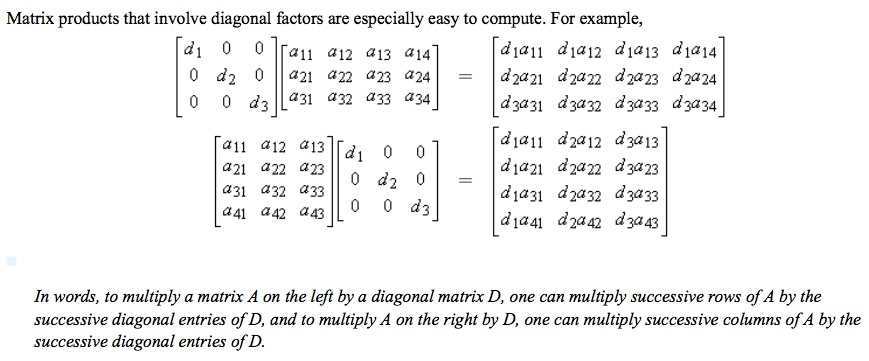
\includegraphics[scale=0.55]{figures_mvc/Mult_by_Diagonal_Matrix}

\begin{exercise}
Let $A=\begin{bmatrix}
	3 & 0 & 0 \\ 0 & 2 & 0 \\ 0 & 0 & 5
\end{bmatrix}, B=\begin{bmatrix}
	-1 & 2 & 0 \\ 5 & 3 & 4 \\ 
\end{bmatrix}, C=\begin{bmatrix}
	5 & 1 & -2 & 3 \\ 1 & 1 & -1 & 0 \\ 
	6 & 2 & 3 & -4
\end{bmatrix}$. Compute $BA$ and $AC$.
\end{exercise}

\subsubsection{Triangular matrices}
	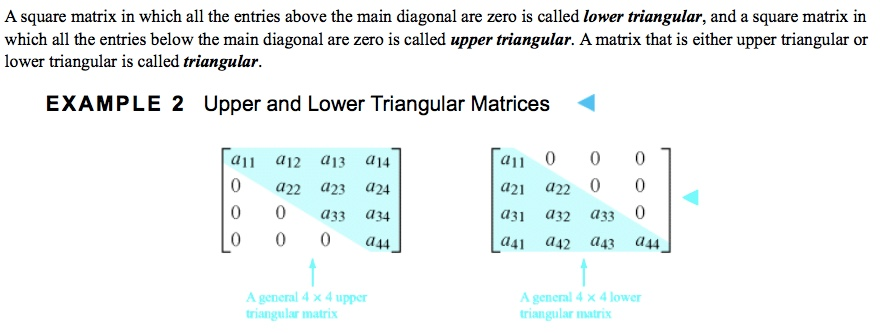
\includegraphics[scale=0.55]{figures_mvc/Triangular_Matrices} 
	
In terms of the matrix elements $a_{ij}$: 
\begin{itemize}
	\item A square matrix is lower triangular if $a_{ij}=0$ for $i<j$.
	\item A square matrix is upper triangular if $a_{ij}=0$ for $i>j$.
\end{itemize}

\begin{thm}[Properties of triangular matrices] \label{thm:properties_of_triangular_matrices} \hspace{10cm}
		\begin{enumerate}[(a)]
	\item If $A$ is lower (upper) triangular, then $A^T$ is upper (lower) triangular.
	\item If $A_1,\cdots, A_k$ are lower (upper) triangular, then so is the product $A_1\cdots A_k$.
	\item A triangular matrix is invertible if and only if its diagonal entries are all nonzero.
	\item If $A$ is an invertible lower (upper) triangular matrix, then so is $A^{-1}$.
	\end{enumerate}
\end{thm}

\begin{pf}
(a) $A$ lower triangular means $a_{ij}=0$ for $i<j$. Since $(A^T)_{ij}=a_{ji}$, $(A^T)_{ij}=0$ for $i>j$, hence $A^T$ is upper triangular. 

(b) Suppose $A$ and $B$ are lower triangular. Then 
\begin{align*}
	(AB)_{ij}=\sum_{k=1}^{n}A_{ik}B_{kj}=\sum_{k=1}^{j-1}A_{ik}\underbrace{B_{kj}}_{=0 \ \forall k}+\sum_{k=j}^{n}\underbrace{A_{ik}}_{=0 \ \forall k}B_{kj}=0.
\end{align*}
The fact that $A_1 A_2 \cdots A_k$ is lower (upper) triangular if $A_1, A_2,\cdots, A_k$ are follows by induction on $k$. 

(c) If $d_j=0$ for some $j$, then the $j$th column would not be a pivot column, so $A$ would not be row-equivalent to $I$ and hence would not be invertible. 

(d) We will prove this later once we have a formula for $A^{-1}$ for a general $n \times n$ invertible matrix.	
\end{pf}

\begin{exercise}
Let $A=\begin{bmatrix}
		1 & 3 & -1 \\ 0 & 2 & 4 \\ 0 & 0 & 5
	\end{bmatrix}, B= \begin{bmatrix}
		3 & -2 & 2 \\ 0 & 0 & -1 \\ 0 & 0 & 1
	\end{bmatrix}$. Compute $A^{-1}, B^{-1}, AB,$ and $BA$.	
\end{exercise}

\subsubsection{Symmetric matrices}
A square matrix $A$ is {\bf symmetric} if $A=A^T$. Some examples are
\begin{align*}
	\begin{bmatrix}
		7 & -3 \\ -3 & 5
	\end{bmatrix}, \begin{bmatrix}
		1 & 4 & 5 \\ 4 & -3 & 0 \\ 5 & 0 & 7
	\end{bmatrix}, \begin{bmatrix}
		d_1 & 0 & 0 & 0 \\ 0 & d_2 & 0 & 0 \\ 0 & 0 & d_3 & 0 \\ 0 & 0 & 0 & d_4
	\end{bmatrix}
\end{align*}
In terms of the matrix elements $a_{ij}$, a matrix is symmetric if $a_{ij}=a_{ji}$ for all $i,j$.
 
\begin{thm}[Properties of symmetric matrices]
		If $A$ and $B$ are symmetric matrices with the same size, and if $k$ is any scalar, then
\begin{enumerate}[(a)] 
	\item $A^T$ is symmetric.
	\item $A+B$ and $A-B$ are symmetric.
	\item $kA$ is symmetric.
	\item If $A$ and $B$ are symmetric, then $AB$ is symmetric if and only if $A$ and $B$ commute.
	\item If $A$ is an invertible symmetric matrix, then $A^{-1}$ is symmetric.
\end{enumerate}
\end{thm}

\begin{pf}
(a) $(A^T)^T=A=A^T$ (since $A$ is symmetric), hence $A^T$ is symmetric. 

(b) $(A+B)^T=A^T+B^T=A+B$.

(c) $(kA)^T=kA^T=kA$. 

(d) $(AB)^T=B^TA^T=BA$. Then $BA=AB \iff A$ and $B$ commute. 

(e) We will prove this later once we have a formula for $A^{-1}$ for a general invertible matrix.	\fixme{Introduce Cramer's rule before this?}
\end{pf}

\subsubsection{$AA^T$ and $A^TA$}
Matrix products of the form $AA^T$ and $A^TA$ arise in a variety of applications. 

\begin{thm}[Properties of $AA^T$ and $A^TA$]\label{thm:props_of_aat_and_ata}
	\begin{enumerate}[(a)]
		\item The products $AA^T$ and $A^TA$ are both square matrices. They are the same size if and only if $A$ is a square matrix.
		\item The products $AA^T$ and $A^TA$ are both symmetric.
		\item If $A$ is invertible, then $AA^T$ and $A^TA$ are also invertible.
	\end{enumerate}
\end{thm}

\begin{pf}
	\begin{enumerate}[(a)]
		\item If $A$ is $m\times n$, $A^T$ is $n \times m$. Therefore $AA^T$ is $m \times m$ and $A^TA$ is $n \times n$. They are the same size iff $n=m$, i.e., if $A$ is a square matrix.
		\item $(AA^T)^T=(A^T)^T(A)^T=AA^T$. $(A^TA)^T=(A)^T(A^T)^T=A^TA$.
		\item $(AA^T)^{-1}=(A^T)^{-1}A^{-1}=(A^{-1})^TA^{-1}$. $(A^TA)^{-1}=A^{-1}(A^T)^{-1}=A^{-1}(A^{-1})^T$.
	\end{enumerate}
\end{pf}

\begin{exercise}
	Let $A=\begin{bmatrix}
		1 & -2 & 4 \\ 3 & 0 & -5
	\end{bmatrix}$. Show explicitly that $A^TA$ and $AA^T$ are symmetric matrices.	
\end{exercise}


\end{document}

